\documentclass[11pt, twocolumn]{article}
\usepackage{titlesec}
\usepackage{tikz}
\usepackage{booktabs}
\usepackage{adjustbox} 
\usepackage{enumitem}
\usepackage{multirow}
\usepackage{bbding,enumitem}
\usepackage{authblk}
\usepackage{fancyhdr}
\usepackage{amsmath}
\usepackage{subcaption}
\usepackage[table]{xcolor}
\setcounter{secnumdepth}{3} % for adjusting padding
\pagestyle{fancy}
\newcommand{\blueoval}{%
    \begin{tikzpicture}[remember picture, overlay]
    \shade[shading=axis, left color=blue, right color=white] (current page.north west) -- (3,0) arc (0:180:4cm) -- cycle;
    \end{tikzpicture}%
}

\newcommand{\coloredfooter}{%
    \begin{tikzpicture}[remember picture, overlay]
    \shade[shading=axis, left color=teal, right color=white] (current page.south east) -- (-1,-2) arc (0:80:2cm) -- cycle;
    \end{tikzpicture}%
}

\fancyhf{} % Clear default header and footer
\fancyhead[L]{ \leftmark}
% Display section title in the left header
\fancyhead[R]{\thepage} % Display page number in the right header
\definecolor{mypink3}{cmyk}{0, 0.7808, 0.4429, 0.1412}

\makeatletter
\renewcommand{\maketitle}{\bgroup\setlength{\parindent}{0pt}
\begin{flushleft}
  \textbf{\@title}

  \@author
\end{flushleft}\egroup
}
\makeatother

\title{\Huge \color{mypink3}{ROV Document}  \vspace{0.5cm}}
\author{\Large E-JUST Robotics Club \normalsize \hspace{0.5cm} }

\setlength{\parindent}{0pt}
\date{\today}

\usepackage[showframe=false, margin=.75in]{geometry}

\usepackage{abstract}
\renewcommand{\abstractname}{}    % clear the title
\renewcommand{\absnamepos}{empty} % originally center

\usepackage{lipsum}

\usepackage{afterpage}

\renewenvironment{abstract}
 {\small
  \begin{center}
  \bfseries \abstractname\vspace{-.5em}\vspace{0pt}
  \end{center}
  \list{}{%
    \setlength{\leftmargin}{10mm}% <---------- Change margin here
    \setlength{\rightmargin}{\leftmargin}%
  }%
  \item\relax}
 {\endlist}

\usepackage[utf8]{inputenc}

%\usepackage{graphicx}
\usepackage{wrapfig}
\usepackage[lofdepth,lotdepth]{subfig}
\usepackage{booktabs}

\usepackage{rotating}

\usepackage{caption}
%\usepackage{subcaption}

%\usepackage[ngerman]{babel}

\usepackage{csquotes}

\setlength{\marginparwidth}{2cm} % Set marginparwidth to avoid todonotes issues
\usepackage{todonotes}

\usepackage{stfloats}

\usepackage[T1]{fontenc}
\usepackage{textcomp}
\usepackage{times}

\usepackage{framed} %um Boxen zu machen

\usepackage[citestyle=authoryear,
			bibstyle=authoryear,
			language=auto,
			url=false,
			backend=bibtex,
			doi=false,
			isbn=false]{biblatex}
	\renewbibmacro*{volume+number+eid}{%
  \printfield{volume}%
%  \setunit*{\adddot}% DELETED
  \setunit*{\addnbspace}% NEW (optional); there's also \addnbthinspace
  \printfield{number}%
  \setunit{\addcomma\space}%
  \printfield{eid}}
\DeclareFieldFormat[article]{number}{\mkbibparens{#1}}

\usepackage{setspace}
\onehalfspacing

\setlength{\columnsep}{0.8cm}

\setlength{\parskip}{0em}

\usepackage{color}
\definecolor{black}{gray}{0} % 10% gray

\usepackage[colorlinks=true,linkcolor=black,citecolor=black]{hyperref}

\usepackage{tabularx}
\newcolumntype{s}{>{\hsize=.5\hsize}X}

\usepackage{ntheorem}
\newtheorem*{TRQ}{Research Question}

\newtheorem{Hyp}{Hypothesis} 

\usepackage{graphicx}
\usepackage{fancyhdr}
\usepackage{lipsum}
\usepackage{geometry}
\usepackage{changepage} % To adjust page margins locally
\usepackage{afterpage}

% Apply the custom header and footer to all pages
\fancyfoot[L]{\hspace*{-1.9cm}{
\includegraphics[width=\paperwidth,height=1.9cm]{1Images/Footer.png}}} % Footer

\pagestyle{fancy}
\makeatletter
\providecommand{\sf@counterlist}{} % Define sf@counterlist to avoid undefined control sequence
\makeatother

\usepackage{titlesec}

\titlespacing*{\subsection}{0pt}{5pt}{5pt}
\titlespacing*{\subsubsection}{0pt}{5pt}{5pt}

\setcounter{secnumdepth}{4}
\renewcommand\theparagraph{\thesubsubsection.\arabic{paragraph}}

\usepackage{tabularray}
\DefTblrTemplate{firsthead,middlehead,lasthead}{default}{}
\DefTblrTemplate{firstfoot}{default}{
  \UseTblrTemplate{contfoot}{default}
  \UseTblrTemplate{caption}{default}
}
\DefTblrTemplate{middlefoot}{default}{
  \UseTblrTemplate{contfoot}{default}
  \UseTblrTemplate{capcont}{default}
}
\DefTblrTemplate{lastfoot}{default}{
  \UseTblrTemplate{note}{default}
  \UseTblrTemplate{remark}{default}
  \UseTblrTemplate{capcont}{default}
}
\DefTblrTemplate{contfoot-text}{default}{Continue on the next column}
\DefTblrTemplate{capcont}{default}{\UseTblrTemplate{caption}{default}}
\UseTblrLibrary{booktabs}
\captionsetup{skip=3pt}
\SetTblrInner{rowsep=0pt, stretch=0.9}
\setlength{\headheight}{13.6pt}
\addtolength{\topmargin}{-1.6pt}
\setlength{\footskip}{58.2pt}

\begin{document}

\tableofcontents

\clearpage


\begin{abstract}
    Hi, this is the abstract O\_\_\O!
\end{abstract}


\section{Design Rationale}

\subsection{Design Evolution}
The development of \textbf{Kamikaze} was the result of a step-by-step design process that began with a critical evaluation of last year’s model, Shiro Kaijin (Figure \ref{fig:shiro_kaijin}). By identifying its limitations, we carefully assessed alternative solutions, ensuring that each design decision balanced performance, cost, and operational efficiency. 

\begin{figure}[h]
    \centering
    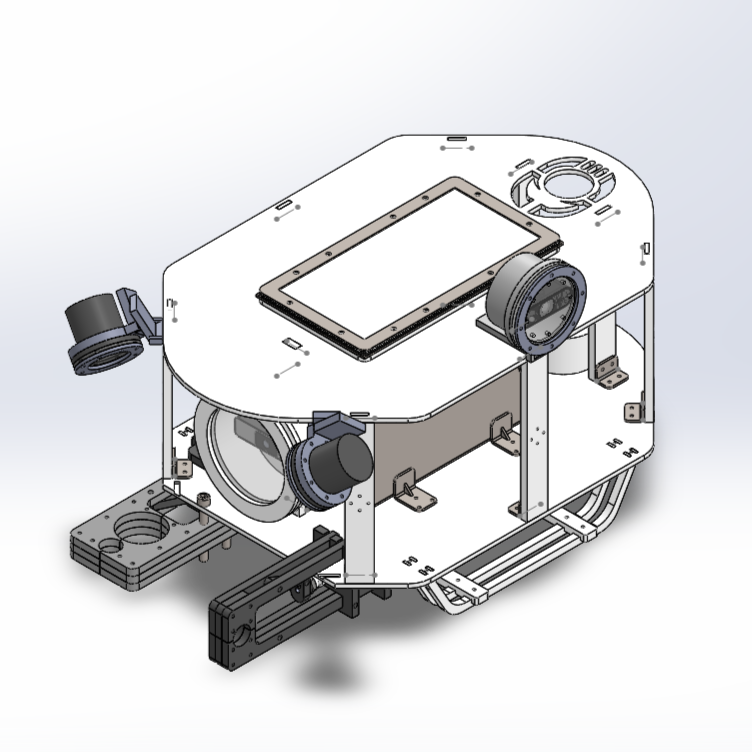
\includegraphics[width=0.7\columnwidth]{Sections/2Design Rationale/images/Shiro Kaijin.png}
    \caption{Last year's ROV - Shiro Kaijin.}
    \label{fig:shiro_kaijin}
\end{figure}

Our team conducted structured brainstorming sessions to explore innovations that would enhance functionality while maintaining cost-effectiveness. Through a holistic systems approach, we ensured seamless integration between mechanical, electrical, and software components, optimizing overall performance. As a result, Kamikaze (Figure \ref{fig:Kamikaze}) represents a well-planned evolution that enhances reliability, efficiency, and mission adaptability.

\begin{figure}[hb!]
    \centering
    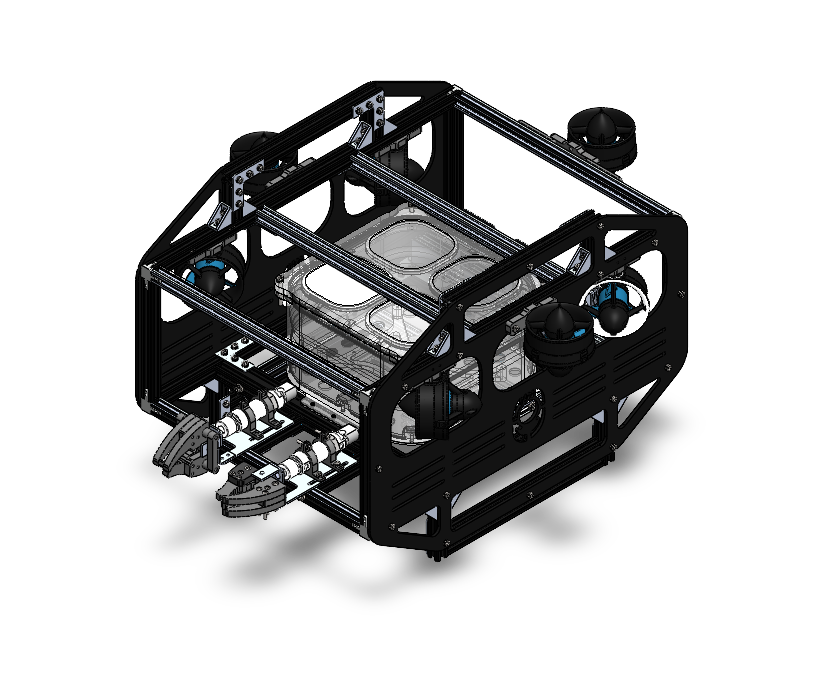
\includegraphics[width=0.7\columnwidth]{Sections/2Design Rationale/images/Kamikaze.png}
    \caption{Kamikaze.}
    \label{fig:Kamikaze}
\end{figure}

\subsubsection{Mechanical System Evolution}
\vspace{0pt}
\textbf{Frame and Structural Improvements}

Shiro Kaijin’s frame was constructed entirely from HDPE, which posed challenges in component fixation. Drilling holes for mounting often led to overlap issues, making modifications difficult. To address this, Kamikaze features a modular aluminum extrusion body, enabling flexible component placement, quick adjustments, and easier repairs.

\vspace{0.2cm}
\textbf{Canister Evolution}

One of the major design advancements in Kamikaze is the transition from an aluminum canister to a 3D-printed PETG canister. While aluminum provided durability, it was costly, difficult to modify, and unnecessarily heavy. The new 3D-printed PETG canister offers greater design flexibility, allowing for customized internal layouts, easy adjustments, and rapid prototyping without the constraints of metal fabrication.

\vspace{0.2cm}
\textbf{Propulsion System}

Kamikaze improves upon its predecessor’s six-thruster configuration by adopting a seven-thruster setup, enhancing maneuverability and control. However, in line with cost-efficiency objectives, all thrusters from last year’s model were reused, maintaining a balance between improved functionality and resource optimization.

\vspace{0.2cm}
\textbf{Gripper Mechanism Enhancement}

Shiro Kaijin’s gripper was limited to fixed circular openings, restricting it to predefined object sizes. Kamikaze introduces a versatile gripping mechanism capable of adapting to various object dimensions, significantly increasing efficiency and flexibility in underwater tasks.

\vspace{0.2cm}
\textbf{Improved Piloting and Camera System}

Kamikaze enhances operational efficiency with an upgraded camera system supporting multiple camera types with rotation and tilt functionality. This ensures a comprehensive, adaptable view of the environment, improving pilot control and situational awareness.

\subsubsection{Electrical System Evolution}

\textbf{Power Connection and Cable Management Issues}

Shiro Kaijin faced instability in power connections due to disorganized cables, causing electrical noise and intermittent connectivity. Each ESC was connected separately, leading to excessive wiring and limited space within the canister. To resolve this, Kamikaze integrates all ESCs into a single PCB, significantly reducing cable clutter, minimizing electrical noise, and improving system stability. Additionally, an STM32 microcontroller was added to the power PCB, further optimizing wiring and ensuring a more reliable electrical system.

\vspace{0.2cm}
\textbf{Inadequacy of Arduino UNO}

The Arduino UNO, used as the main controller, struggled to handle multiple sensors, leading to irregular data handling and performance issues. Kamikaze replaces it with an STM32 microcontroller, offering better stability, higher processing power, and improved efficiency for industrial applications. 

\vspace{0.2cm}
\textbf{CAN Bus Integration}

To further enhance system communication, a CAN bus was integrated, enabling reliable data exchange between multiple STM32s, reducing wiring complexity, and allowing independent node resets without affecting the overall system. This implementation ensures robust and efficient communication, critical for the seamless operation of Kamikaze's various subsystems.

\vspace{0.2cm}
\textbf{Limitations of MS5540 Depth Sensor}

The MS5540 depth sensor was inaccurate, slow, and costly, making it an inefficient choice. Kamikaze replaces it with a custom-designed depth sensor, providing real-time, accurate measurements and better connectivity options. To improve monitoring capabilities, voltage and current sensors were also implemented, allowing precise tracking of power consumption and early detection of system faults.

\vspace{0.2cm}
\textbf{Reliability of Main Control PCB}

Shiro Kaijin used relays in the main control PCB, which affected system stability. Kamikaze replaces them with MOSFETs, enhancing reliability and improving performance. Additionally, a debugging node using the W5500 Ethernet module was introduced, enabling real-time system monitoring and remote reset of multiple nodes, ensuring stability and efficient troubleshooting.

\vspace{0.2cm}
\textbf{Switching from Copper to Aluminum Wires}

Copper wires in high-power transmission corroded quickly, posing safety risks. Kamikaze replaces them with aluminum wires, which are lighter, more durable, and resistant to redox reactions, ensuring safer and more efficient power transmission.

\subsubsection{Software System Evolution}

\textbf{ZED Camera}

This year, we added a stereo camera to our ROV to enhance our navigation capabilities. The ZED2i camera is capable of providing depth perception and 3D mapping, which can be utilized in Task 1: Shipwreck length estimation. We exploited epipolar geometry algorithms to be able to estimate the length of the ship from the depth data provided. We believe that this addition is crucial to the development of our ROV, and it's a decent investment for the future. \\

\vspace{0.2cm}
\textbf{$\boldsymbol{\mu}$ROS}

We improved our communication model even more by the integration of micro-ROS, a ROS 2 implementation for microcontrollers, on one of the STM32 we have. We used micro-ROS Ethernet to connect the STM32 to the top-side computer, which is running ROS 2, allowing for seamless integration between the microcontrollers and the main computer. Micro-ROS ensures real-time communication and efficient data exchange, enhancing the overall performance of our ROV.   

% For now we don't need images - Shaheen
% \begin{figure}[h]
%     \centering
%     \rule{0.8\columnwidth}{4cm}
%     \caption{Software System Evolution.}
%     \label{fig:software_system}
% \end{figure}

\subsection{Design and Manufacturing Process}

\subsubsection{Conceptual Design}

The design process began with a comprehensive evaluation of last year’s ROV to identify areas for improvement. The team focused on two primary aspects: performance optimization and the integration of new features required for this year’s tasks.

\hspace{10pt} To ensure a structured approach, brainstorming meetings were conducted to analyze feasibility, cost, and impact on overall performance. One of the major innovations was the adoption of a modular aluminum extrusion body, a strategic decision aimed at enhancing adaptability and extending the ROV’s lifespan. 

\hspace{10pt} Another key challenge was selecting suitable material for the electronic canister. An aluminum design was initially considered but was found to be twice as expensive as a 3D-printed alternative. After evaluating material strength and pressure resistance, the team decided to proceed with 3D printing, ensuring a cost-effective and flexible solution that could withstand underwater conditions while being easy to assemble and modify.

\subsubsection{Preliminary Design}

Once the core design concepts were defined, SolidWorks simulations were conducted to evaluate structural integrity, hydrodynamics, and thruster configurations. These data-driven insights played a critical role in optimizing component placement and material selection.

\hspace{10pt} To ensure an optimal balance between performance and affordability, a trade-off matrix (Figure \ref{fig:material_selection}) was developed, comparing materials based on weight, cost, and manufacturability. Additionally, build vs. buy decisions were assessed, ensuring that in-house manufacturing was pursued where it provided a functional and economic advantage, while outsourcing was considered for components requiring specialized fabrication.

\begin{figure}[h]
    \centering
    \rule{0.8\columnwidth}{4cm}
    \caption{Material Selection}
    \label{fig:material_selection}
\end{figure}

\hspace{10pt} To validate these theoretical analyses, small-scale prototypes were developed for key components. The 3D-printed canister was tested for sealing effectiveness, and successful trials confirmed its reliability before moving to full-scale manufacturing. Camera housings were also prototyped to optimize field-of-view placement. This iterative process allowed for practical verification of design choices before finalizing the ROV.

\subsubsection{Detailed Design and Manufacturing}

With validated designs, the final ROV model (Figure \ref{fig:kamikaze_drawings}) was fully developed in SolidWorks, incorporating stress, buoyancy, and flow simulations to ensure structural stability and hydrodynamic efficiency.

\begin{figure}[h]
    \centering
    \rule{0.8\columnwidth}{4cm}
    \caption{Kamikaze Drawings}
    \label{fig:kamikaze_drawings}
\end{figure}

For manufacturing, a systems-based approach was taken:

\vspace{-0.5\baselineskip}
\begin{itemize}
    \setlength{\itemsep}{0pt}
    \item The aluminum plates body was Laser CNC-machined and assembled using precise modular connectors.
    \item The canister was made using 3D printing, with design improvements tested through simulation and prototype experiments.
    \item The grippers and other HDPE parts were cut using router cutters, leveraging precise CAD models to minimize material waste. 2D CAD models (Figure \ref{fig:dxf}) were generated to optimize material usage.
\end{itemize}

\begin{figure}[h]
    \centering
    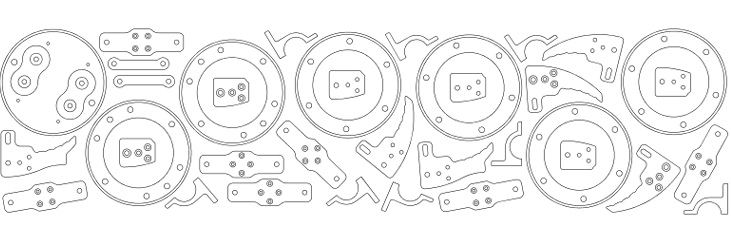
\includegraphics[width=0.8\columnwidth]{Sections/2Design Rationale/images/DXF.png}
    \caption{DXF file for cutting the float and grippers.}
    \label{fig:dxf}
\end{figure}

For the electrical system, significant innovations were implemented:

\vspace{-0.5\baselineskip}
\begin{itemize}
    \setlength{\itemsep}{0pt}
    \item The ESCs were integrated into a single PCB, reducing wiring complexity, electrical noise, and space consumption within the canister. This improvement streamlined system integration and enhanced overall performance. (Figure \ref{fig:pcb})
    \item A custom-designed depth sensor replaced the previous board, offering higher accuracy, real-time measurements, and expanded connectivity options. This upgrade ensured more precise and reliable depth control.
\end{itemize}

\begin{figure}[h]
    \centering
    \rule{0.8\columnwidth}{4cm}
    \caption{PCB}
    \label{fig:pcb}
\end{figure}

Finally, the complete ROV assembly was tested to ensure seamless integration of mechanical, electrical, and software components.

\subsection{Vehicle Core Systems}
\subsubsection{Mechanical System}

\paragraph{Frame} \ \\
\vspace{-0.5cm}

Kamikaze’s frame (Figure \ref{fig:frame}) is designed using a cuboid aluminum V-extrusion structure, providing a stable and modular foundation for mounting various components. The 20×20 and 20×40 aluminum extrusions offer a strong yet lightweight framework that maintains structural integrity in underwater conditions.

\hspace{10pt} To enhance stability and buoyancy, HDPE side frame sheets (Figure \ref{fig:side_frame}) are integrated into the design. These sheets not only contribute to the aesthetic appeal of the ROV but also help in maintaining balance during operations. Their strategic placement ensures that the ROV remains hydrodynamically stable while supporting the overall structural framework.

\hspace{10pt} The frame is designed with precise mounting slots, allowing secure positioning of thrusters, cameras, and operational tools while maintaining easy access for maintenance. The bolted assembly ensures that components can be reconfigured or replaced without permanent modifications.

\hspace{10pt} Additionally, the frame is tailored for the E-JUST Robotics team, ensuring compatibility with the mission requirements of the MATE ROV competition while balancing durability, weight efficiency, and adaptability.

\begin{figure}[t]
    \centering
    \begin{subfigure}[b]{0.45\columnwidth}
        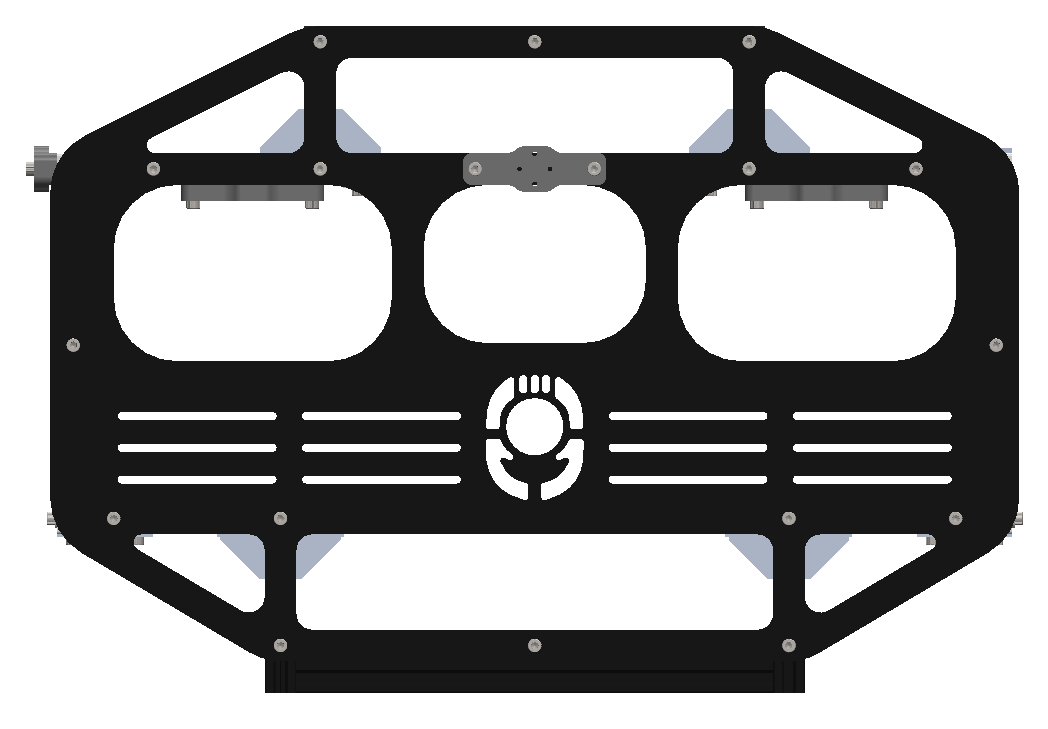
\includegraphics[width=\textwidth]{Sections/2Design Rationale/images/side frame.png}
        \caption{HDPE Side Frame.}
        \label{fig:side_frame}
    \end{subfigure}
    \hfill
    \begin{subfigure}[b]{0.5\columnwidth}
        \includegraphics[width=\textwidth]{Sections/2Design Rationale/images/frame.png}
        \caption{Aluminum Extrusion Frame.}
        \label{fig:frame}
    \end{subfigure}
    \caption{Kamikaze's Frame Illustration.}
    \label{fig:full_frame}
\end{figure}

\vspace{-0.3cm}
\paragraph{Propulsion} \ \\
\vspace{-0.5cm}

Kamikaze is equipped with seven T200 Blue Robotics thrusters, strategically placed to achieve six degrees of freedom for precise maneuverability (Figure \ref{fig:dof}). This setup balances performance, power consumption, and cost-efficiency, ensuring mission success without excessive energy use.

\hspace{10pt} Using seven thrusters instead of a larger number reduces power draw while maintaining stability and control. Each thruster's power consumption is affected by drag force, given by:

\begin{equation}
    F_d = \frac{1}{2} C_d \rho A v^2
    \label{eq:drag_force}
\end{equation}

Where:

\vspace{-0.5\baselineskip}
\begin{itemize}
    \setlength{\itemsep}{0pt}
    \item \(F_d\) = Drag force (N)
    \item \(C_d\) = Drag coefficient (ROV shape-dependent)
    \item \(\rho\) = Water density (kg/m\(^3\))
    \item \(A\) = Cross-sectional area (m\(^2\))
    \item \(v\) = ROV velocity (m/s)
\end{itemize}

\begin{figure}[h]
    \centering
    \includegraphics[width=\columnwidth]{Sections/2Design Rationale/images/dof.png}
    \caption{Kamikaze’s Degrees of Freedom.}
    \label{fig:dof}
\end{figure}

A CFD flow simulation was conducted to analyze water flow around Kamikaze (Figure \ref{fig:cfd}), minimizing drag and enhancing hydrodynamic efficiency.

\begin{figure}[b]
    \centering
    \rule{0.8\columnwidth}{4cm}
    \caption{Flow Simulation.}
    \label{fig:cfd}
\end{figure}

\vspace{0.2cm}
\textbf{Trade-offs in Thruster Selection}
\vspace{-0.5\baselineskip}
\begin{itemize}
    \setlength{\itemsep}{0pt}
    \item \textbf{Power vs. Performance:} More thrusters improve stability but increase power consumption. Seven thrusters provide a balance between efficiency and control.
    \item \textbf{Cost vs. Mission Needs:} Reusing last year’s T200 thrusters reduces costs while still meeting competition requirements.
\end{itemize}

\vspace{-0.3cm}
\paragraph{Buoyancy and Stability} \ \\
\vspace{-0.5cm}

Something about buoyancy and stability. \lipsum[1]

\begin{figure}[h]
    \centering
    \rule{0.8\columnwidth}{4cm}
    \caption{Buoyancy.}
    \label{fig:buoyancy}
\end{figure}

\vspace{-0.3cm}
\paragraph{Main Canister} \ \\
\vspace{-0.5cm}

The canister serves as the primary enclosure for the ROV, protecting essential components such as microcontrollers, power systems, and sensors while ensuring pressure resistance, corrosion protection, and ease of maintenance. The design consists of a 3D-printed PETG body, an aluminum base, and a PETG lid with embedded acrylic windows, providing structural stability and waterproof integrity under operational conditions.

\begin{figure}[h]
    \centering
    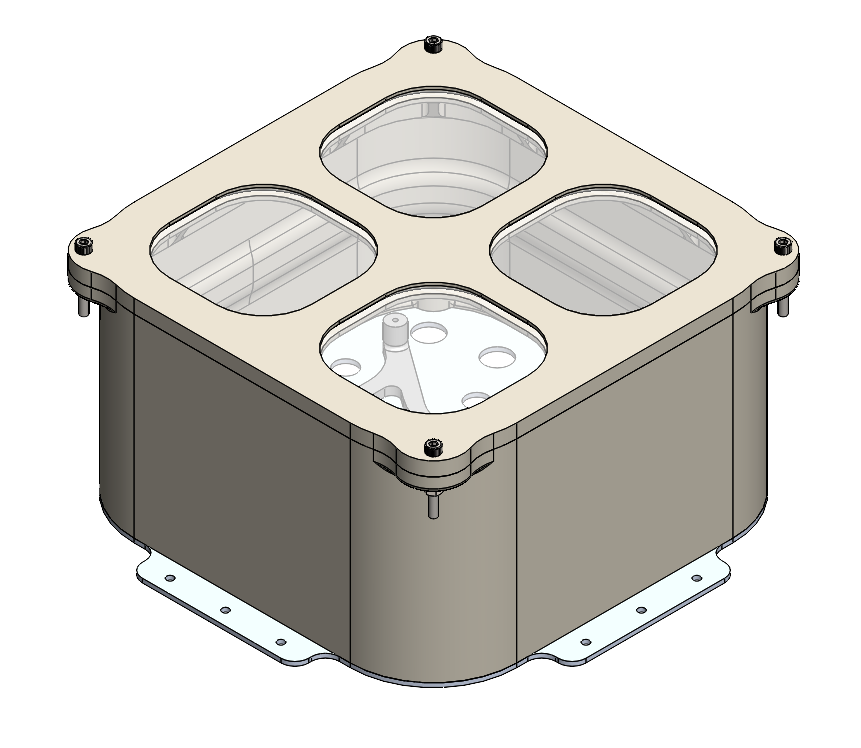
\includegraphics[width=0.6\columnwidth]{Sections/2Design Rationale/images/canister.png}
    \caption{Kamikaze’s Main canister.}
    \label{fig:canister}
\end{figure}

\hspace{10pt} PETG was chosen as a cost-effective alternative to aluminum, offering a balance between mechanical strength and manufacturability. Although PETG is inherently waterproof, Sikadur®-31 CF sealant was applied to enhance structural integrity and reliability. The 3mm-thick aluminum base provides structural support for bulkhead glands, preventing layer separation and ensuring durability. The canister dimensions are 276×276×142.59 mm, optimized for component housing and pressure resistance. A three-stage sealing process was implemented, consisting of mechanical fastening, epoxy bonding, and polyurethane sealant, to maintain a watertight enclosure. The removable PETG lid, secured with M5 screws and dual O-rings, allows for easy inspection and maintenance, while four embedded acrylic windows provide visual access without disassembly.

\hspace{10pt} To evaluate structural performance, a Finite Element Analysis (FEA) was conducted:

\vspace{-0.5\baselineskip}
\begin{itemize}
    \setlength{\itemsep}{0pt}
    \item \textbf{Top View (Figure \ref{fig:top_fda}):} Stress is concentrated around circular openings and edges, which experience higher mechanical loads from water pressure.
    \item \textbf{Bottom View (Figure \ref{fig:bottom_fda}):} Bolted connections and interface zones between the base and side walls accumulate stress, making them susceptible to deformation.
\end{itemize}

\begin{figure}[h]
    \centering
    \begin{subfigure}[b]{0.45\columnwidth}
        \rule{\textwidth}{4cm}
        \caption{Top View Analysis.}
        \label{fig:top_fda}
    \end{subfigure}
    \hfill
    \begin{subfigure}[b]{0.45\columnwidth}
        \rule{\textwidth}{4cm}
        \caption{Bottom View Analysis.}
        \label{fig:bottom_fda}
    \end{subfigure}
    \caption{Main Canister Finite Element Analysis.}
    \label{fig:fda}
\end{figure}

\vspace{-0.3cm}
\paragraph{Sealing Strategy} \ \\
\vspace{-0.5cm}

Waterproofing is critical for the ROV’s performance and durability. The sealing approach protects electronic components while maintaining structural integrity under varying pressures. This design integrates 3D-printed PETG, aluminum, high-performance adhesives, and mechanical fasteners for optimal sealing efficiency.

\vspace{0.2cm}
\textbf{Main Canister Sealing (Electronics Housing)}

\vspace{-0.5\baselineskip}
\begin{itemize}
    \setlength{\itemsep}{0pt}
    \item Sikadur-31 CF adhesive prevents micro-gaps.
    \item IP68-rated metallic cable glands ensure watertight cable entry.
    \item Epoxy resin \& super glue reinforce adhesion.
    \item Bolted fastening ensures long-term stability.
\end{itemize}

\textbf{ZED Camera Enclosure}

\vspace{-0.5\baselineskip}
\begin{itemize}
    \setlength{\itemsep}{0pt}
    \item O-ring in a groove forms a primary seal.
    \item RTV Gasket Maker provides additional waterproofing.
    \item Compression sealing \& Allen bolts apply uniform pressure.
    \item Sikadur-31 CF protects against water exposure.
    
\end{itemize}

\textbf{Artelon Camera Enclosures}

For other cameras, Artelon enclosures replace aluminum.

\vspace{-0.5\baselineskip}
\begin{itemize}
    \setlength{\itemsep}{0pt}
    \item Acrylic cover sandwiched with an O-ring seal ensures water resistance.
    \item Allen bolts provide tight compression for long-term sealing.
\end{itemize}

\textbf{Bolt Spacing Calculation for Optimal Sealing}

To ensure optimal sealing pressure and prevent gasket deformation under load, the bolt spacing (C) is calculated based on flange stiffness, gasket pressure, and deflection using equation \ref{eq:bolt_spacing}.

\begin{equation} \label{eq:bolt_spacing}
    C = \left[ \frac{480 \left( \frac{a}{b} \right) E t^3 \Delta H}{13 P_{\text{min}} + 2 P_{\text{max}}} \right]^{1/4}
    \end{equation}
    where:
    \vspace{-0.5\baselineskip}
    \begin{itemize}
        \setlength{\itemsep}{0pt}
        \item \(C\) = Bolt spacing (mm)
        \item \(a\) = Width of the flange plate (mm)
        \item \(b\) = Width of the gasket (mm)
        \item \(E\) = Modulus of elasticity of the flange material (Pa or N/m\(^2\))
        \item \(t\) = Thickness of the flange (mm)
        \item \(\Delta H\) = Max. gasket deflection - Min. gasket deflection (mm)
        \item \(P_{\text{min}}\) = Minimum gasket pressure (Pa or N/m\(^2\))
        \item \(P_{\text{max}}\) = Maximum gasket pressure (Pa or N/m\(^2\))
    \end{itemize}
    

\vspace{-0.3cm}
\paragraph{Cameras} \ \\
\vspace{-0.5cm}

Something about cameras. \lipsum[1]

\begin{figure}[h]
    \centering
    \rule{0.8\columnwidth}{4cm}
    \caption{Cameras.}
    \label{fig:cameras}
\end{figure}

\vspace{-0.3cm}
\paragraph{Grippers} \ \\
\vspace{-0.5cm}

Two claw grippers (Figure \ref{fig:grippers}) are designed to handle various item shapes and diameters. They are constructed from 10mm HDPE for durability and aluminum for fixation, ensuring a lightweight yet sturdy design. The grippers are pneumatically actuated using a 25mm stroke piston that applies 113–135N of force in both forward and backward directions. With a maximum opening width of 70mm, they can securely grip all required competition objects.

\begin{figure}[h]
    \centering
    \begin{subfigure}[b]{0.49\columnwidth}
        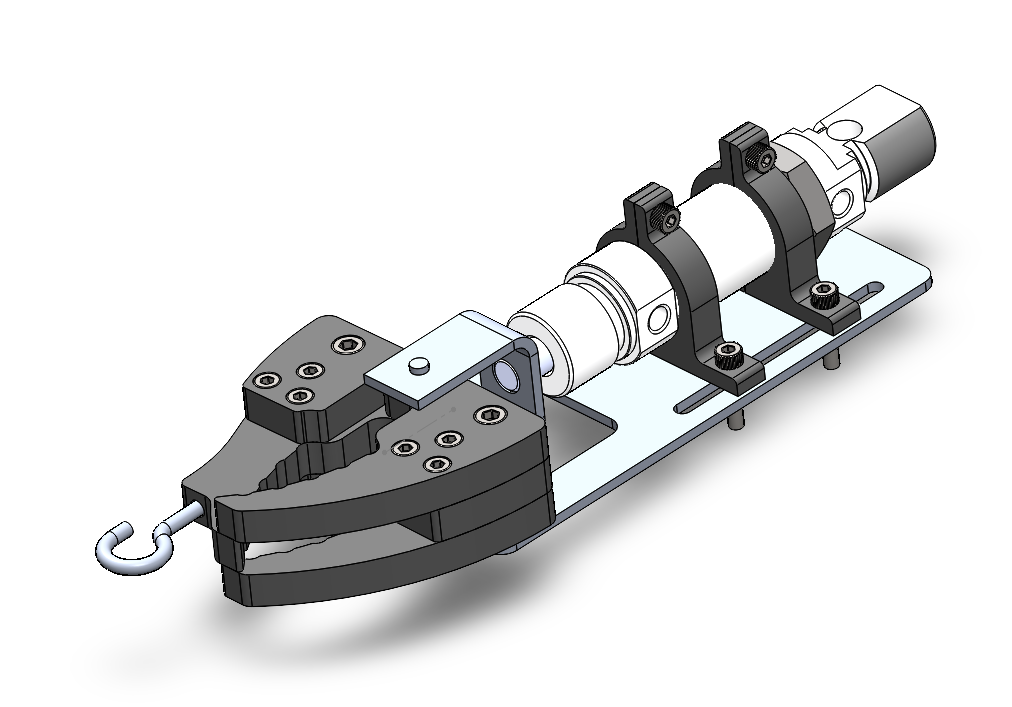
\includegraphics[width=\textwidth]{Sections/2Design Rationale/images/Horizontal.png}
        \caption{Horizontal Gripper.}
        \label{fig:horizontal_gripper}
    \end{subfigure}
    \hfill
    \begin{subfigure}[b]{0.49\columnwidth}
        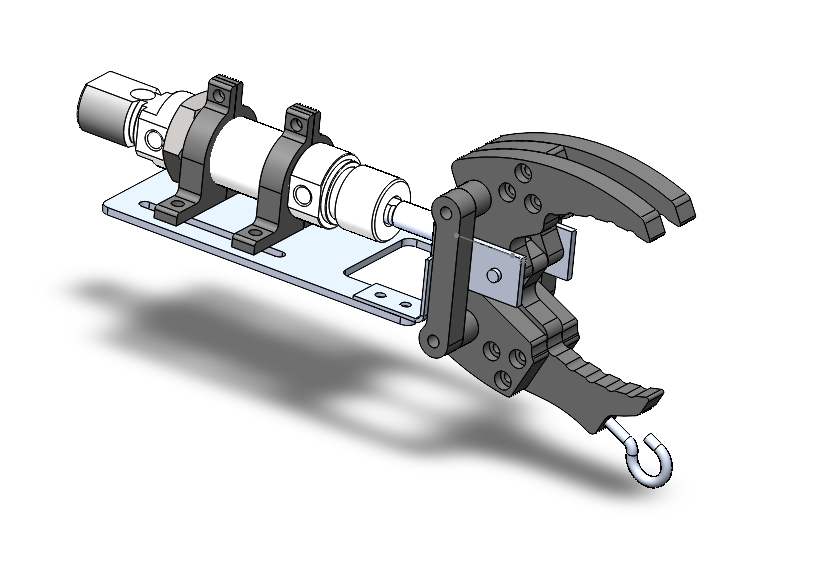
\includegraphics[width=\textwidth]{Sections/2Design Rationale/images/Vertical.png}
        \caption{Vertical Gripper.}
        \label{fig:vertical_gripper}
    \end{subfigure}
    \caption{Kamikaze Grippers.}
    \label{fig:grippers}
\end{figure}

To enhance functionality, two screw hooks were integrated, enabling the ROV to lift hooks and manipulate ropes, expanding its operational capabilities.To optimize the gripper’s design and prevent potential bending stress-induced failures, a comprehensive stress analysis was performed. This theoretical evaluation ensured the gripper’s ability to withstand the designated weight. The results \ref{fig:grippers_analysis}confirmed that:

\vspace{-0.5\baselineskip}
\begin{itemize}
    \setlength{\itemsep}{0pt}
    \item The horizontal gripper can hold up to 14.6 kg.
    \item The vertical gripper can hold up to 11.8 kg.
    \item Both with a safety factor of 2.
\end{itemize}

\begin{figure}[h]
    \centering
    \begin{subfigure}[b]{0.49\columnwidth}
        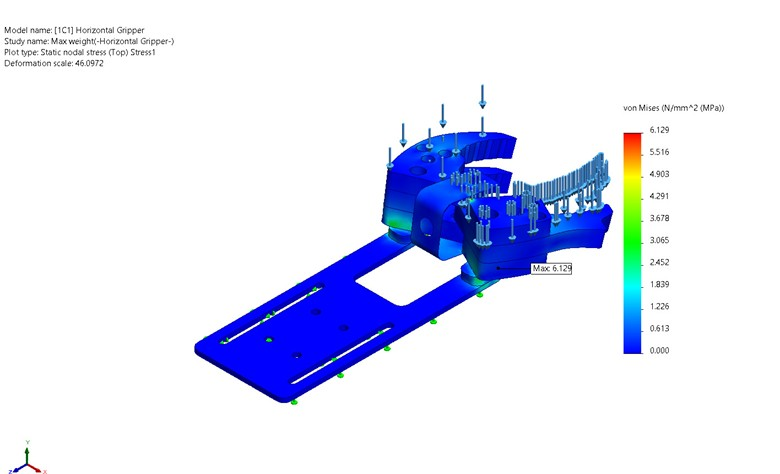
\includegraphics[width=\textwidth]{Sections/2Design Rationale/images/Horizontal Max weight.jpg}
        \caption{Horizontal Gripper Analysis.}
        \label{fig:horizontal_gripper_max_weight}
    \end{subfigure}
    \hfill
    \begin{subfigure}[b]{0.49\columnwidth}
        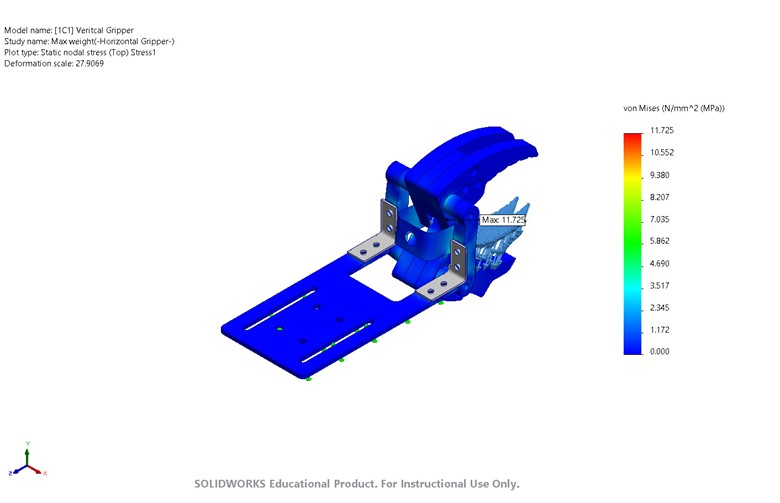
\includegraphics[width=\textwidth]{Sections/2Design Rationale/images/Vertical max weight.jpg}
        \caption{Vertical Gripper Analysis.}
        \label{fig:vertical_gripper_max_weight}
    \end{subfigure}
    \caption{Kamikaze Grippers Analysis.}
    \label{fig:grippers_analysis}
\end{figure}

\subsubsection{Electrical System}

\paragraph{Control Units} \ \\
\vspace{-0.5cm}

\vspace{-\baselineskip}
\begin{enumerate}[label=(\roman*)]
    \setlength{\itemsep}{0pt}
    \item \textbf{Topside Control Unit}
    \item \textbf{Sensors}
    \item \textbf{Underwater Control Unit}
    \item \textbf{System Integration}
\end{enumerate}

\paragraph{Electric Power} \ \\
\vspace{-0.5cm}

\vspace{-\baselineskip}
\begin{enumerate}[label=(\roman*)]
    \setlength{\itemsep}{0pt}
    \item \textbf{Power Conversion System}
    \item \textbf{Power Unit}
\end{enumerate}

\paragraph{Tether} \ \\
\vspace{-0.5cm}

\subsubsection{Software System}

\paragraph{Communication System} \ \\
\vspace{-0.5cm}
The ROV's communication architecture which is illustrated in Figure 1 can be divided into two parts: the top side control unit and the ROV unit.

\begin{figure}[ht]
    \centering
    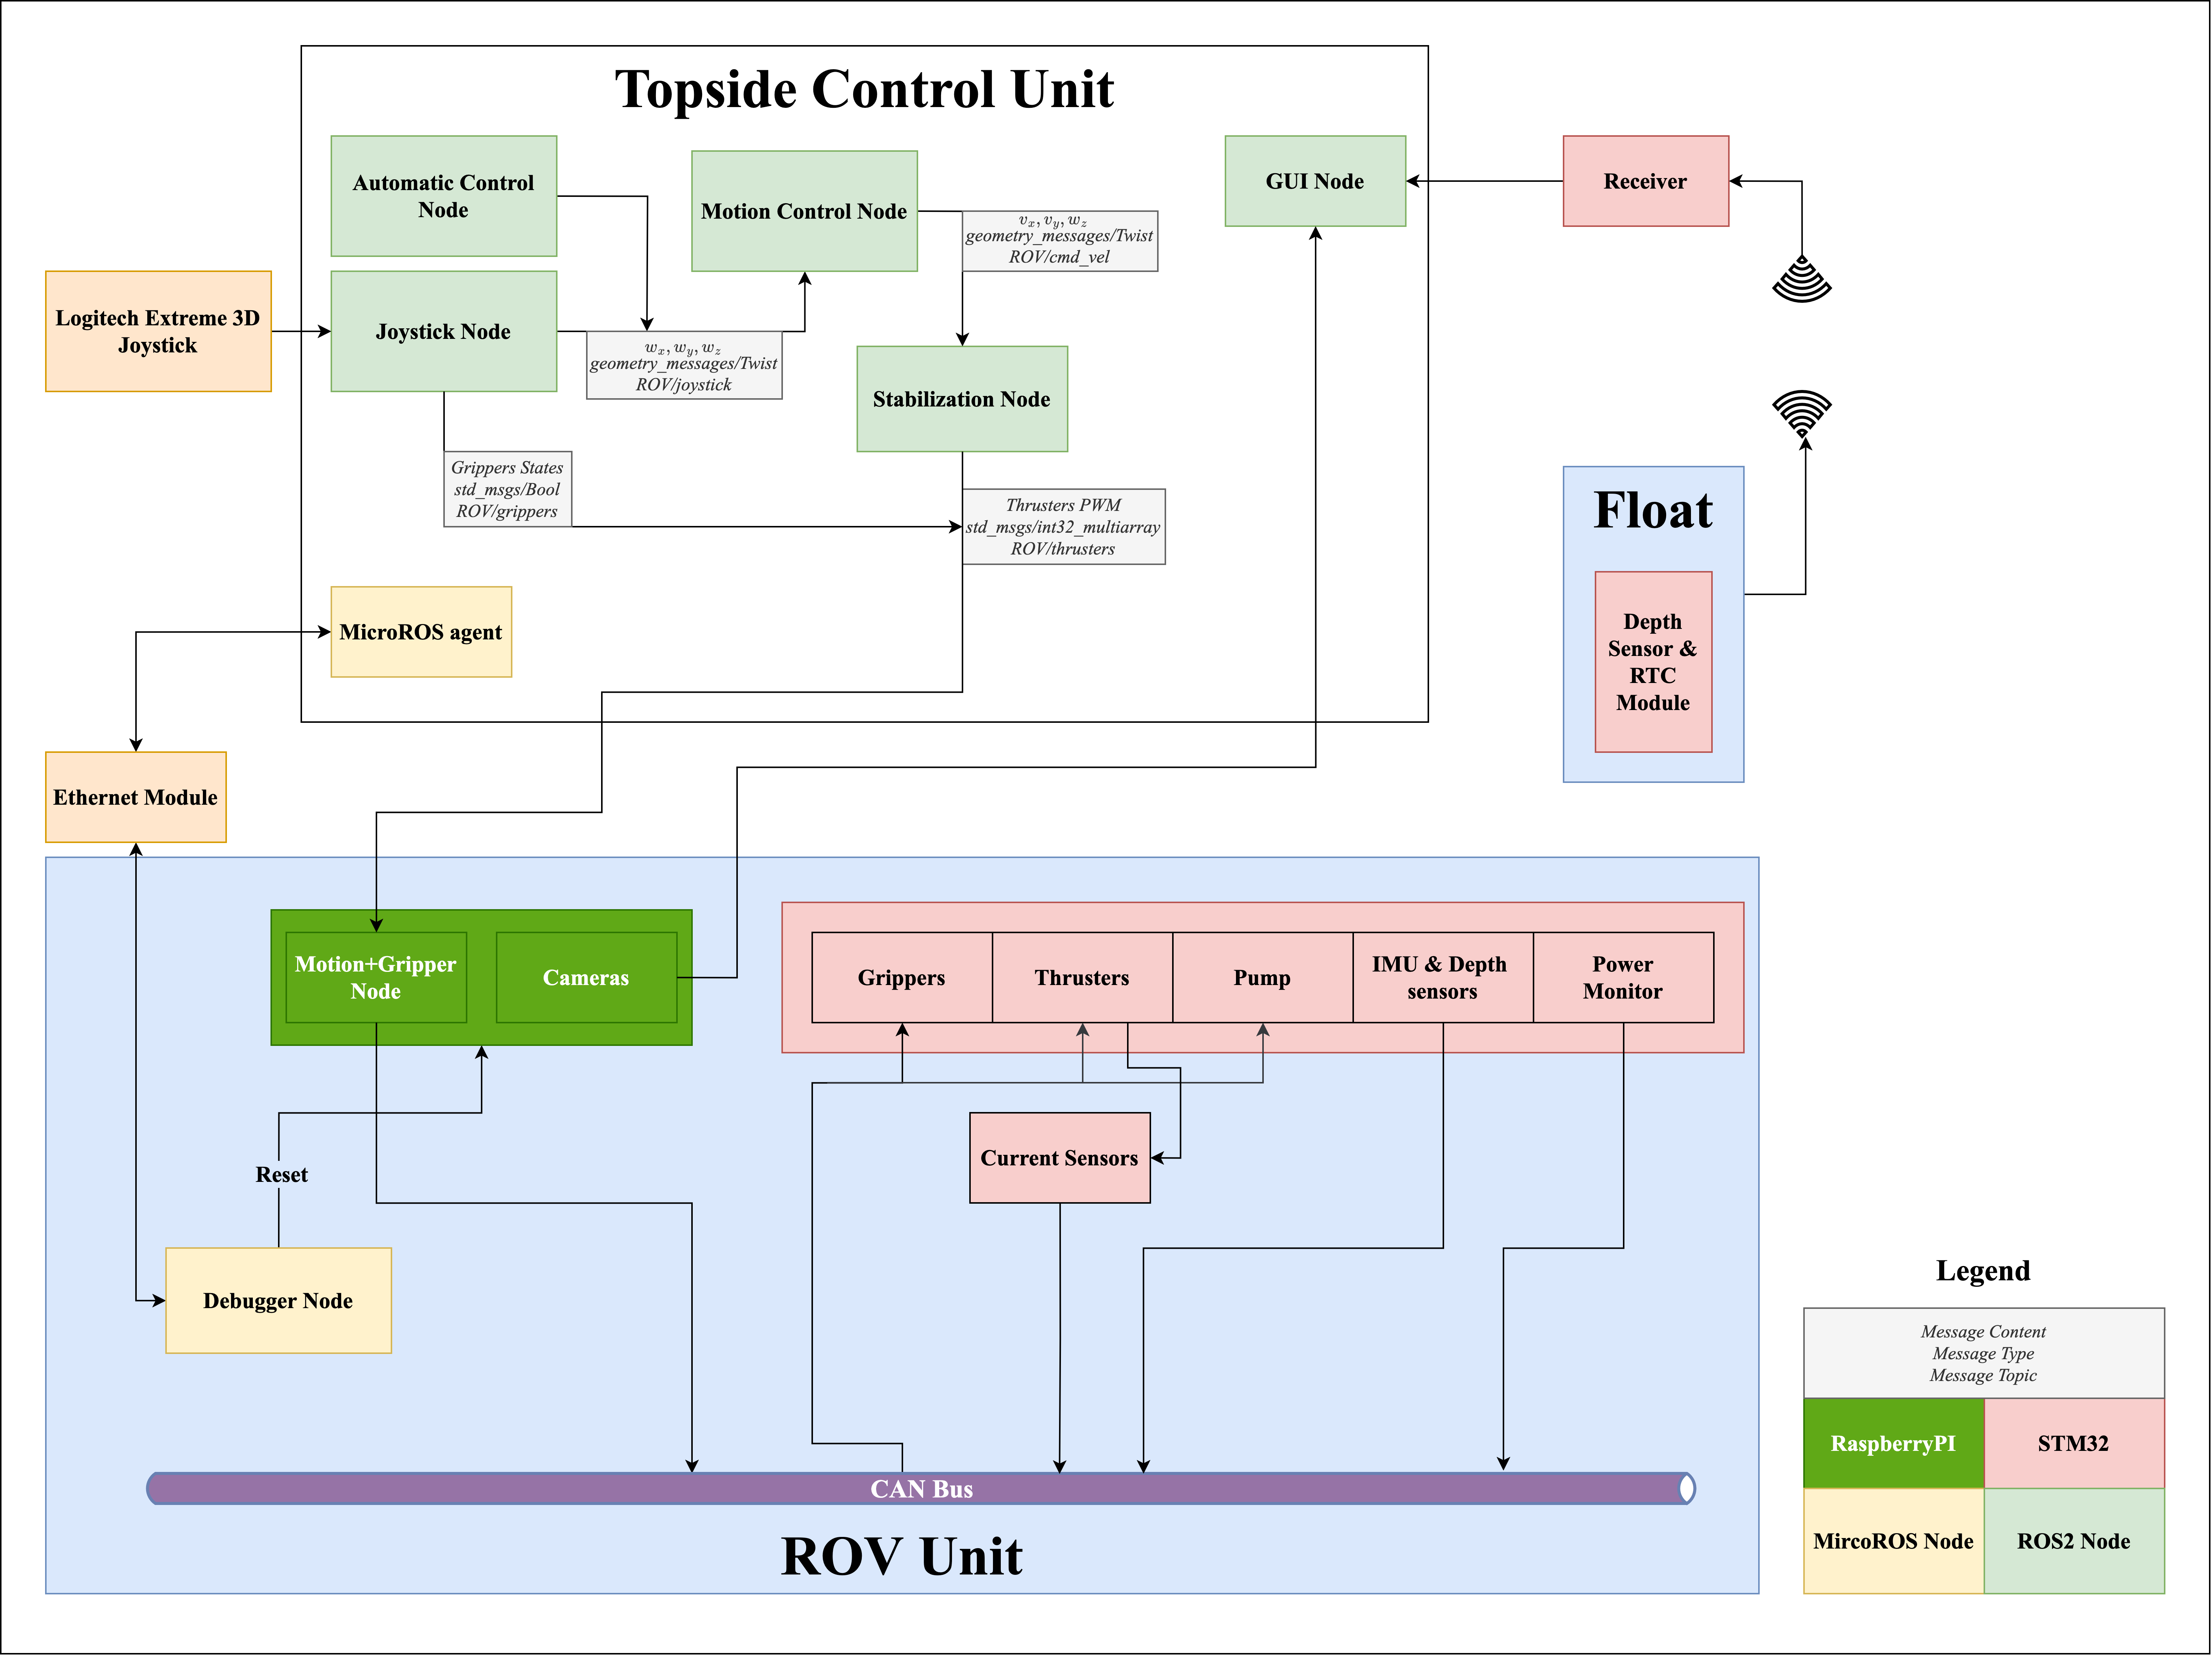
\includegraphics[width=1\linewidth]{rov_architecture_2.png}
    \caption{Communication architecture}
\end{figure}

\vspace{0.2cm}
\textbf{System Evolution and Communication Backbone}

In last year's architecture, we utilized ROS 1 as the main framework for communication between the control unit and the ROV's micro-controllers. 

Communication with MCUs was handled through \texttt{rosserial}, which introduced a critical limitation: the presence of a single point of failure—the ROS Master. Any instability or failure in the master would cause the entire system to halt, making it unreliable in underwater environments where robustness is essential.

\vspace{0.5em}
This year, we have transitioned fully to ROS 2, eliminating the dependency on a centralized master. Communication between the topside control unit and the ROV unit is now handled using ROS2 \& CAN communication, which is more reliable, scalable, and real-time capable.
\vspace{0.5em}


In parallel, we’ve integrated \texttt{micro-ROS} to run a debugger node on the ROV side. This node communicates with the topside unit via an Ethernet module, acting as a backup communication path. In the event of failure of our SBC—the Raspberry Pi, this channel ensures continued monitoring of the entire system's vitals which greatly facilitates debugging in case of a problem with our system.

\vspace{0.5em}
This upgraded architecture enhances reduces the risk of total system failure, making it far more suitable for mission-critical underwater operations and industrial applications.

\vspace{0.2cm}
\textbf{Topside Control Unit}
The topside control unit hosts the nodes and agents that work above water which includes:
\begin{itemize}
    \item Joystick Node
    \item Automatic Control Node
    \item Stabilization Node
    \item Motion Control Node 
    \item GUI Node
    \item Micro-ROS agent
\end{itemize}
Data is received from the following streams:
\begin{itemize}
    \item Camera feed from the ZED camera as well as the side-assisting cameras
    \item Readings from sensors which includes an IMU sensor and a depth sensor
    \item Readings from the joystick
    \item Receiver from the Float unit
\end{itemize}
The joystick node is interfaced with the Logitech Extreme 3D Pro Joystick, capturing signals and converting them into ROS messages, which then are sent over to the motion control node in order to order to convert these signals to motion vectors and gripper operations. 

For autonomous tasks, the automatic control node is pivotal. It receives commands from the joystick and autonomously sends out commands to the motion control node.

The motion control node converts the received messages into motion vectors that are then sent to the stabilization node.

The stabilization node is used to maintain the operational stability of the ROV by applying various PID controllers to counter any disturbances.

The GUI node acts as the pilot's interface, displaying camera feeds for navigation as well as displaying the ROV's vitals.

Vitals include: 
\begin{itemize}
    \item IMU readings
    \item Depth readings from both the ROV unit and the Float unit
    \item Thrusters PWM values
\end{itemize}

\vspace{0.2cm}
\textbf{ROV Unit}
The ROV unit is where a lot of the heavy lifting happens, it executes commands received from the topside control unit, streams cameras and hosts the debugger node.

The ROV unit has a Raspberry Pi 5 that's responsible for streaming cameras to the GUI node as well as it hosts a ROS 2 node that is responsible for receiving the commands from the stabilization node.

Connected to the Raspberry Pi 5 is the CAN bus where it receives data from sensors such as current sensors, a depth sensor, an IMU and the power monitor.
That are then published to both the topside control unit as well as the debugger node.

\vspace{0.2cm}
\textbf{Float Unit}
The float unit hosts a depth senor that transmits it's readings using an NRF transceiver module and an RTC (Real-time Clock) to the receiver which are then displayed on the GUI in the topside control unit.

\vspace{-0.3cm}
\paragraph{Graphical User Interface} \ \\
Our GUI prioritizes stability, usability, and responsiveness, balancing personalization with default configurations. Built with Python and PyQt5, it ensures a stable and efficient desktop experience.

\vspace{0.2cm}
\textbf{System Architecture}
The GUI follows a modular design, dividing functionality across four interfaces: Pilot, Copilot, Engineer, and Float. This enhances maintainability while tailoring tools to each role.

\vspace{0.2cm}
\textbf{Pilot Interface}
Designed for minimal clutter, the Pilot interface displays five camera feeds essential for navigation. To ensure smooth streaming, we use Python's \texttt{Multiprocessing} library, preventing latency and glitches. The Pilot can switch views and resize feeds as needed. Our redundant streaming system prevents a single point of failure—if one camera disconnects, others remain functional. 

\vspace{0.2cm}
\textbf{Copilot Interface}
The Copilot interface extends camera controls, allowing real-time brightness, contrast, and backlight adjustments for varying underwater conditions. It also displays telemetry data, including six degrees of freedom (Vx, Vy, Vz, Roll, Pitch, Yaw), depth, and thruster speeds, aiding in system monitoring and troubleshooting. A screenshot of the interface is shown in Figure \ref{fig:copilot_interface}.

\begin{figure}[ht]
    \centering
    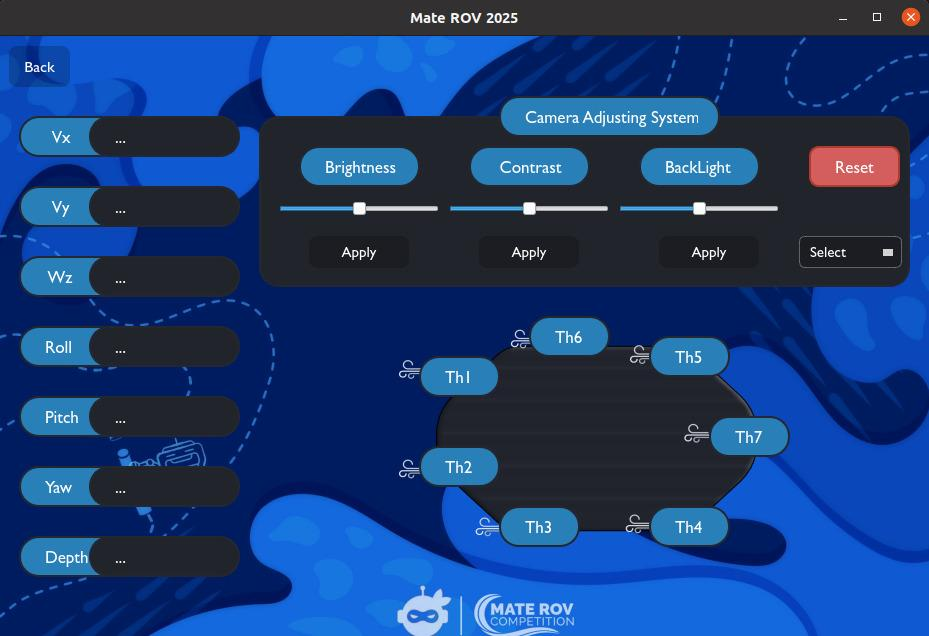
\includegraphics[width=0.8\columnwidth]{Sections/2Design Rationale/images/Copilot_interface.jpeg}
    \caption{Screenshot of the Copilot interface.}
    \label{fig:copilot_interface}
\end{figure}

\vspace{0.2cm}
\textbf{Engineer Interface}
The Engineer interface provides quick access to automation scripts for tasks like invasive carp detection and depth estimation. It also facilitates seamless media capture for Photosphere documentation. All functions are integrated within the GUI, streamlining workflow without external tools. A screenshot of the interface is shown in Figure \ref{fig:Engineer_interface}.

\begin{figure}[h]
    \centering
    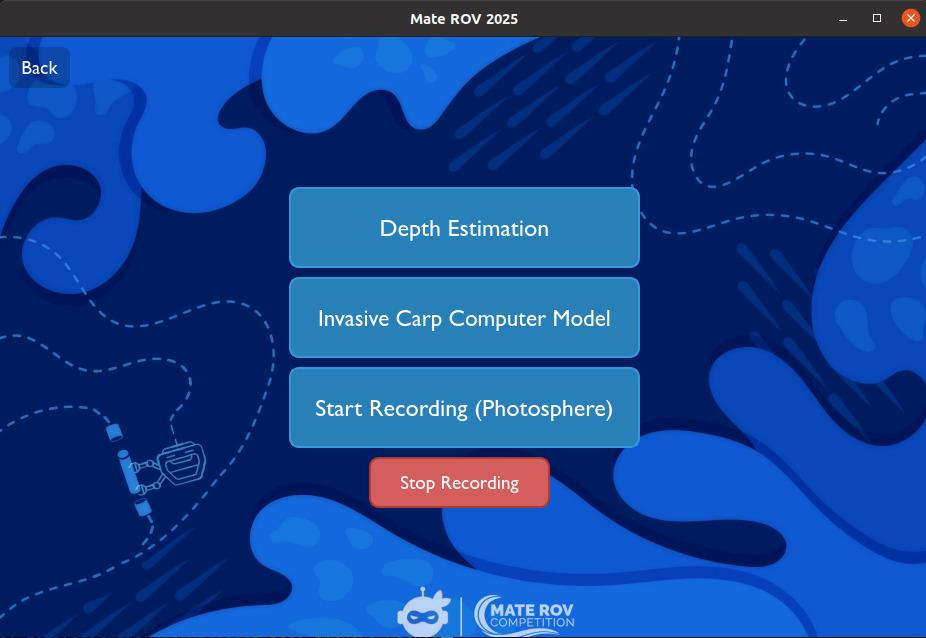
\includegraphics[width=0.8\columnwidth]{Sections/2Design Rationale/images/Engineer_interface.jpeg}
    \caption{Screenshot of the Engineer interface.}
    \label{fig:Engineer_interface}
\end{figure}

\vspace{0.2cm}
\textbf{Float Interface}
The Float interface enables communication with the float before vertical profiling begins and displays depth data along with additional metrics post-profile.

\vspace{-0.3cm}
\paragraph{Kinematics} \ \\
The Kamikaze's movement underwater may be one of the most important aspects of the design. We had to ensure stability, maneuverability, and speed. We achieved this by focusing on two main aspects:

\vspace{-0.5\baselineskip}
\begin{itemize}[leftmargin=0pt, itemindent=10pt]
    \setlength{\itemsep}{0pt}   
    \item \textbf{Thrusters Configuration:} We employed a seventh thruster this year to improve the robot's maneuverability as shown in figure \ref{fig:thruster}. With the current vectored thrusters configuration and this new thruster, we can achieve motion in 6 degrees of freedom. This novel configuration may be the first of its kind to allow for such a wide range of motion while only using 7 thrusters.
    \begin{figure}[h]
        \centering
        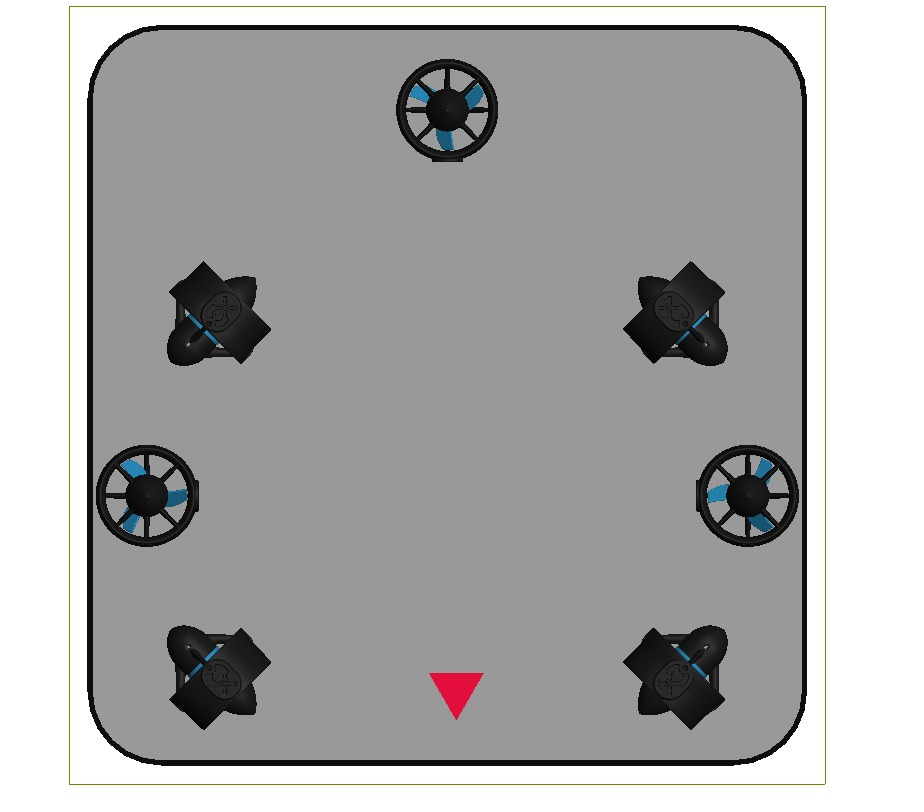
\includegraphics[width=0.8\columnwidth]{Sections/2Design Rationale/images/Thrusters.png}
        \caption{Thruster Configuration}
        \label{fig:thruster}
    \end{figure}

    \item \textbf{PID Control:} We have implemented PID controllers for all critical movement axes, allowing for precise control over the robot's movement and ensures that it remains stable in the water. We implemented an FFT (Fast Fourier Transform) based auto-tuning algorithm to tune the PID parameters, as this is our first year using the new Vehicle. We also supplemented the algorithm with a live
    plotting feature, shown in figure \ref{fig:pid_live}, to allow for manual adjustments to the PID parameters.
    \begin{figure}[h]
    \centering
    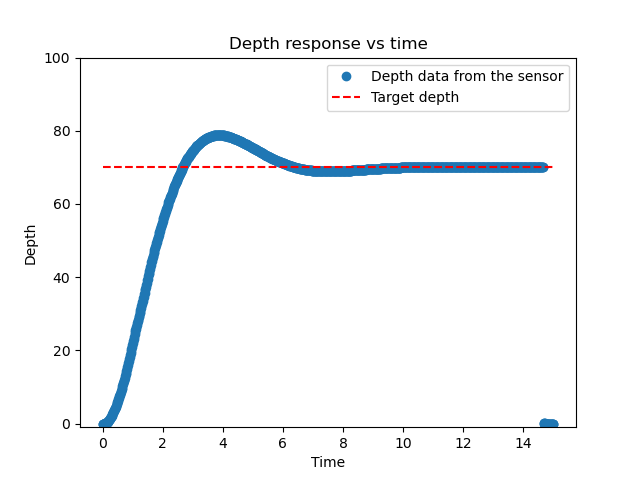
\includegraphics[width=\columnwidth]{Sections/2Design Rationale/images/Pid.png}
    \caption{Live Plotting of PID Parameters}
    \label{fig:pid_live}
    \end{figure}
\end{itemize}

\vspace{-1cm}
\paragraph{Open Sourcing the Kamikaze} \ \\
We have all of our working code available on our GitHub repository. A lot of effort was made this year to maintain, document, and clean up the code, making it easier for future teams to understand and build upon. We believe that this is a crucial step in the development of the Kamikaze, as it allows for a more collaborative environment and ensures that the knowledge gained from each year is not lost. 

\paragraph{Some third point} \ \\
\vspace{-0.5cm}






\subsection{Mission Specific Auxiliary Tools}

\subsubsection{Stabilizing Cap Positioning Extension}

One of the specialized systems developed for Kamikaze is the Stabilizing Cap Positioning Extension (SCPE). While Kamikaze installs a new thermistor, the SCPE (Figure \ref{fig:scpe}) secures the thermistor cap in place, ensuring perfect alignment.

\hspace{10pt} The mechanism's smooth and controlled extension is provided by a telescopic ball-bearing slide, which is like those found in drawer runners. A 2.5-inch diameter cup at the top provides a little amount of alignment tolerance, guaranteeing a firm but flexible hold on the cap.

\hspace{10pt} The extension lengthens as the SCPE holds onto the cap and Kamikaze lowers, keeping the cap in place. The extension shrinks as Kamikaze rises with the thermistor, holding the cap firmly in place and facilitating a smooth hookup.

\subsubsection{Liquid Sample Acquiring System}

To enable efficient and flexible liquid sample collection, a modular design approach (Figure \ref{fig:pump}) was implemented. This design allows for straightforward assembly, disassembly, and maintenance of individual components, thereby improving both convenience and system reliability during the sampling process. To further ensure optimal functionality under high-pressure conditions, the system incorporates a mini pump with a flow rate of 80 L/h, which was tested underwater to validate its performance. Additionally, a collection bottle featuring a user-friendly disassembly mechanism was integrated, easing the sample retrieval process and confirming its compatibility within the overall system.

\subsubsection{Jelly Collecting Shutter Mechanism}

A specialized mechanism has been developed to collect and transport a jelly-like object filled with water to the surface. The system consists of a sealed acrylic tube, closed at the top, with a pneumatically controlled shutter at the bottom. When the pilot successfully guides the jelly inside the tube, the shutter activates, preventing it from drifting away while allowing water to flow freely. This design (Figure \ref{fig:jelly}) ensures that the jelly remains contained within the tube as it ascends due to buoyancy, enabling controlled and efficient transport to the surface.

\subsubsection{Customized Hook}

A customized hook mechanism has been developed to efficiently collect chenille strips (pipe cleaners) from the water surface. Since the strips float on the surface, they cannot be gripped using the ROV’s main gripper. Positioned at the top of the ROV, the hook (Figure \ref{fig:hook}) is strategically designed to maximize the number of strips gathered in a single attempt. To further enhance the mechanism’s effectiveness, Velcro can be added to ensure the strips stick within the hook securely. This design improves the ROV’s efficiency in completing the task, ensuring a higher collection rate.

\begin{figure}[hb!] 
    \centering
    \begin{subfigure}[b]{0.49\columnwidth} 
        \centering
        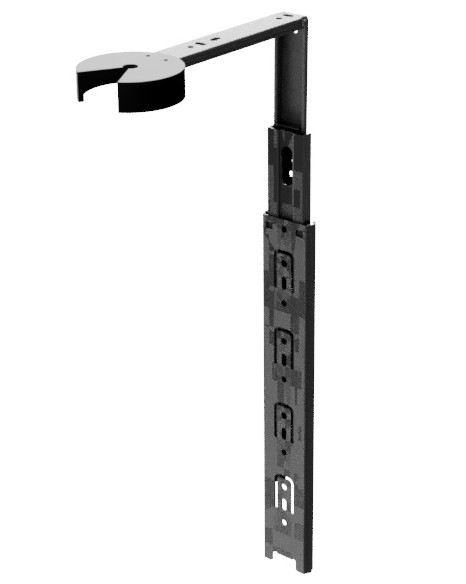
\includegraphics[height=3cm]{Sections/2Design Rationale/images/Stabilizing Cap Positioning Extension (SCPE) .jpg}
        \caption{\scriptsize Stabilizing Cap Positioning Extension.}
        \label{fig:scpe}
    \end{subfigure}
    \hfill
    \begin{subfigure}[b]{0.49\columnwidth}
        \centering
        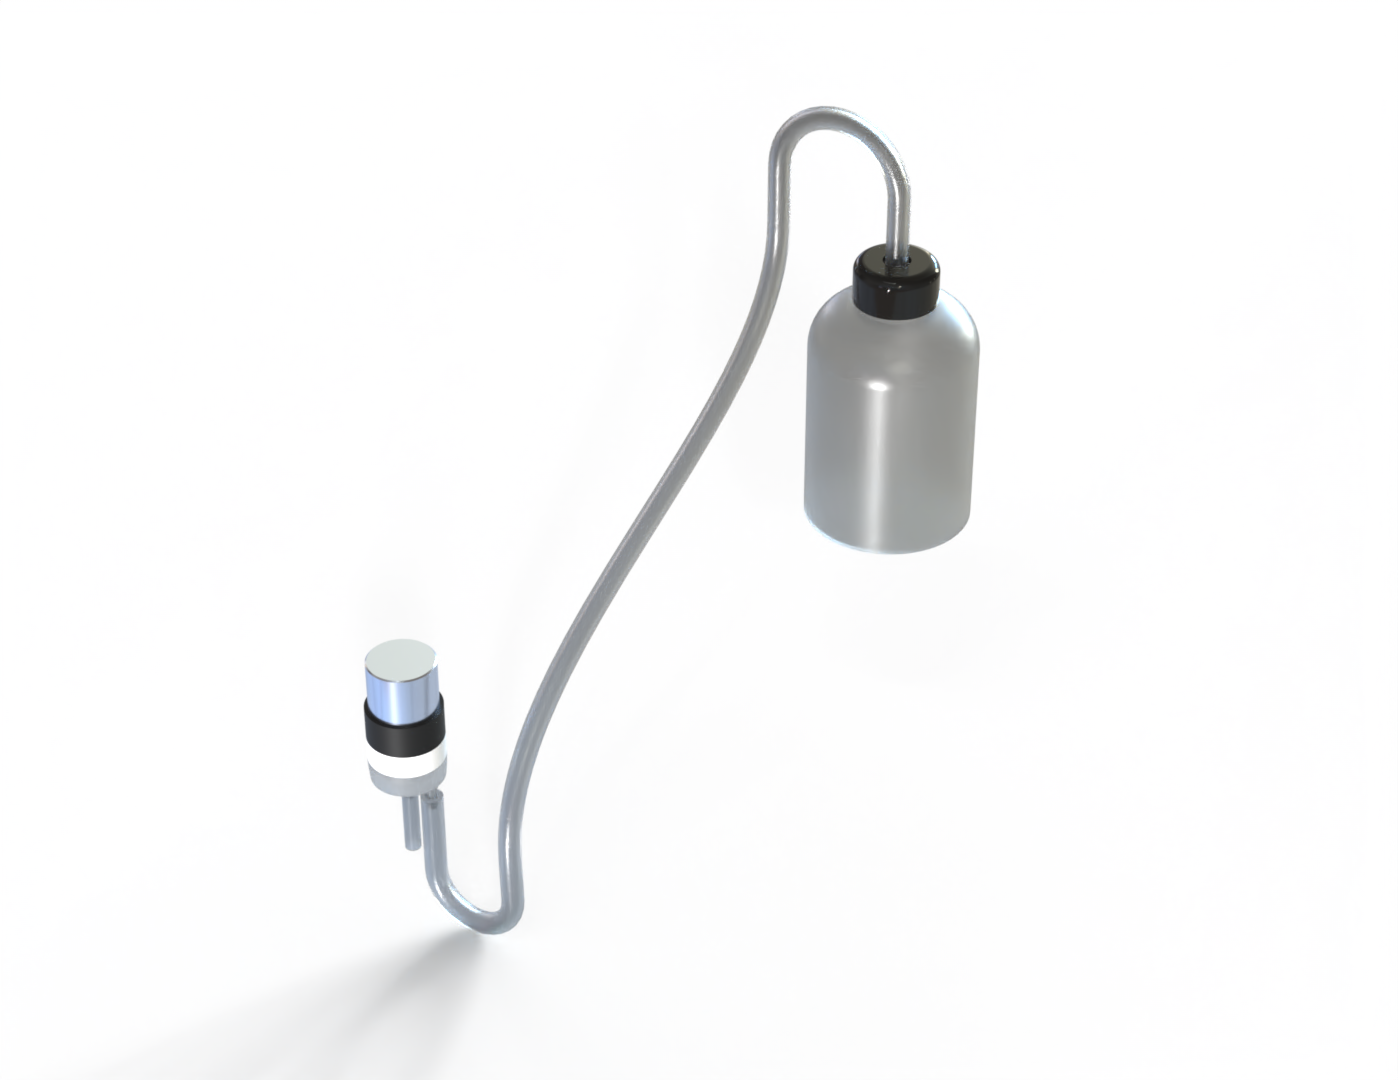
\includegraphics[width=\linewidth]{Sections/2Design Rationale/images/Pump.png}
        \caption{\scriptsize Liquid Sample Acquiring System.}
        \label{fig:pump}
    \end{subfigure}

    \vspace{0.2cm}

    \begin{subfigure}[b]{0.49\columnwidth}
        \centering
        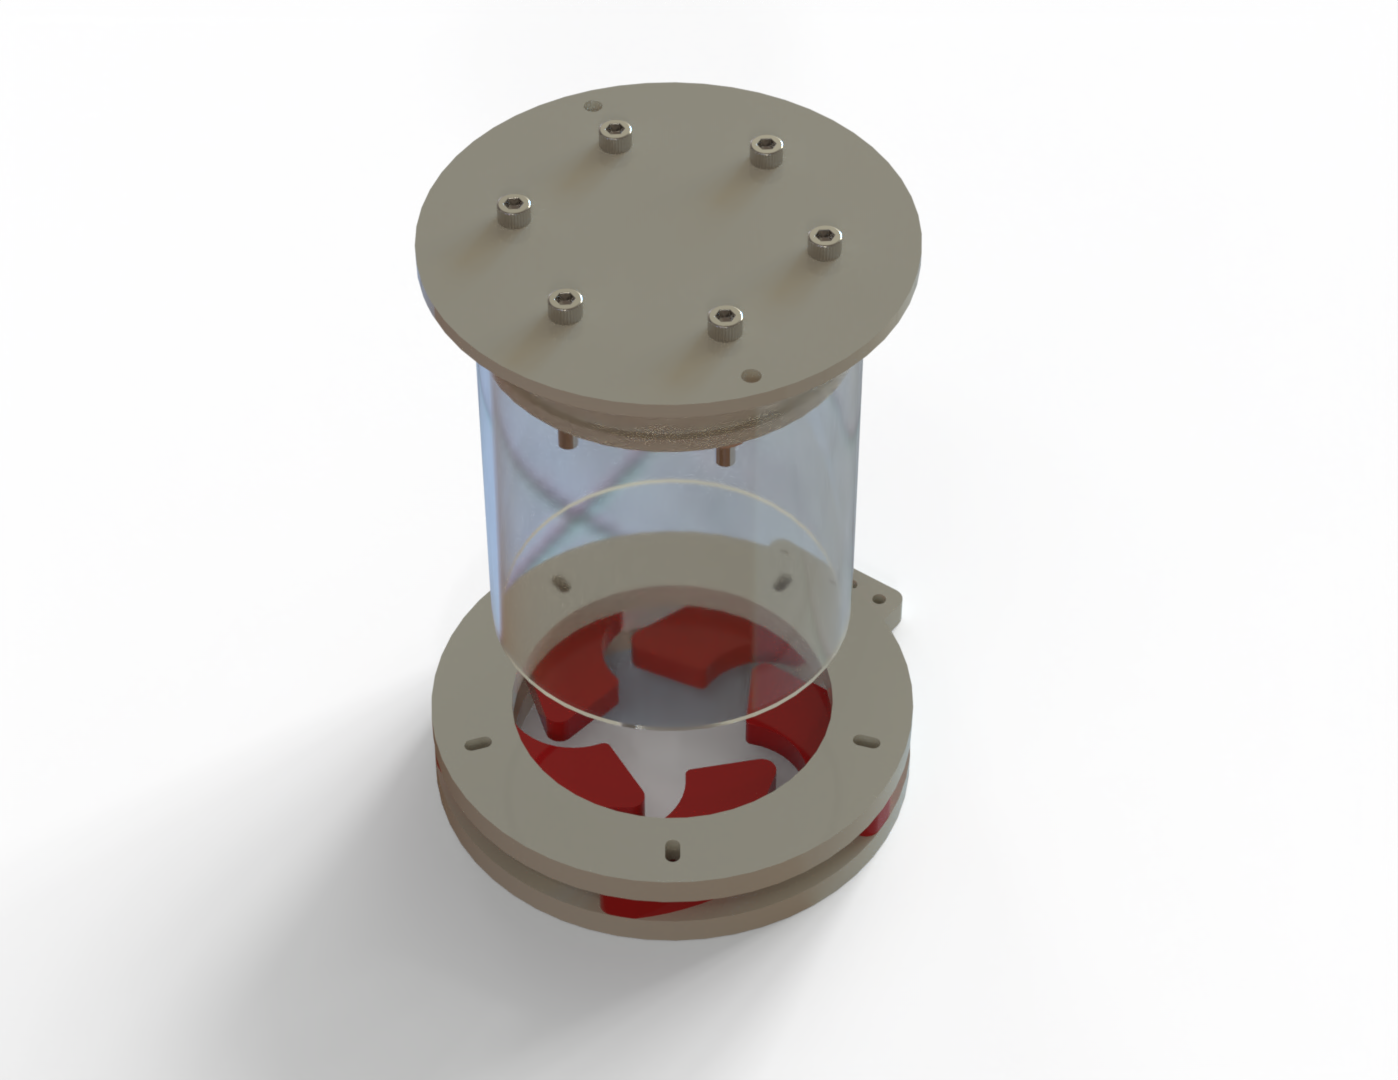
\includegraphics[width=\linewidth]{Sections/2Design Rationale/images/Jelly.png}
        \caption{\scriptsize Jelly Collecting Shutter Mechanism.}
        \label{fig:jelly}
    \end{subfigure}
    \hfill
    \begin{subfigure}[b]{0.49\columnwidth}
        \centering
        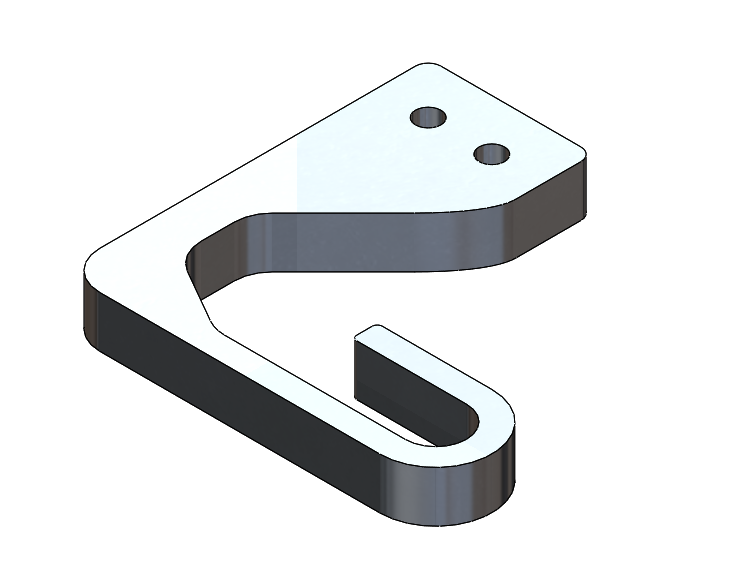
\includegraphics[width=\linewidth]{Sections/2Design Rationale/images/Hook.png} 
        \caption{\scriptsize Customized Hook.}
        \label{fig:hook}
    \end{subfigure}

    \caption{Kamikaze's Mission-Specific Tools.}
    \label{fig:mission_specific_tools}

\end{figure}

\subsubsection{Vertical Profiling Float}

EJUST Robotics Clun supports the National Science Foundation (NSF)-funded GO-BGC project’s mission to build a global network of chemical and biological sensors for ocean health monitoring. As part of this initiative, our team has developed Fat Man, a vertical profiling float designed for ocean observation and data collection. This float enhances the ability to monitor key environmental parameters, providing valuable insights into ocean dynamics and contributing to global research efforts on climate change.

\begin{figure}[h]
    \centering
    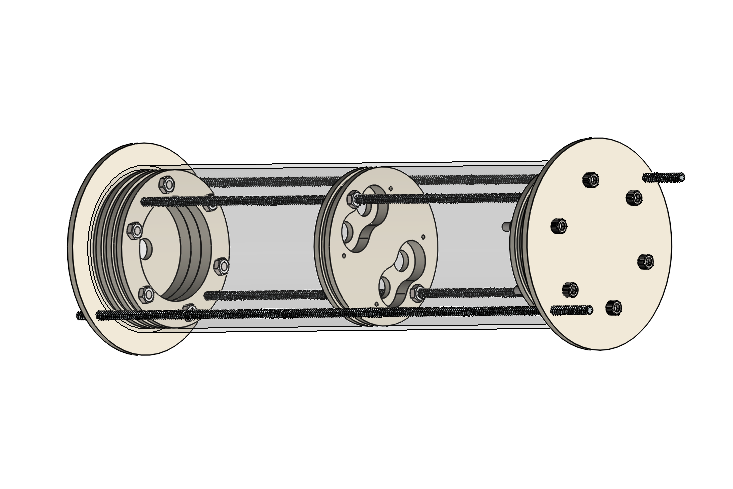
\includegraphics[height=9cm]{Sections/2Design Rationale/images/float.png}
    \caption{E-JUST Vertical Profiling Float, Fat Man.}
    \label{fig:Float}
\end{figure}

\vspace{-0.3cm}
Fat Man is constructed from transparent acrylic, allowing visual inspection and error detection, and is divided into two sections by an HDPE disk to separate the electrical components from the water chamber. A suction system with peristaltic pumps enables precise buoyancy control by regulating water intake and release. The electrical system, powered by an STM32 microcontroller, integrates a depth sensor, motor driver, and NRF24L01 radio module for real-time data collection and transmission. Supported by NiMH batteries, the system ensures stable operation, reinforcing EJUST Robotics Club's commitment to advancing ocean research and technology.

\vspace{-1.5cm}
\section{Safety}

\vspace{-0.3cm}
\subsection{Safety Philosophy}

At E-JUST Robotics Club, safety is the foundation of every aspect of Kamikaze ROV’s design, construction, and operation. We are committed to preventing injuries, protecting equipment, and ensuring a secure working environment for all team members.

\begin{figure}[h]
    \centering
    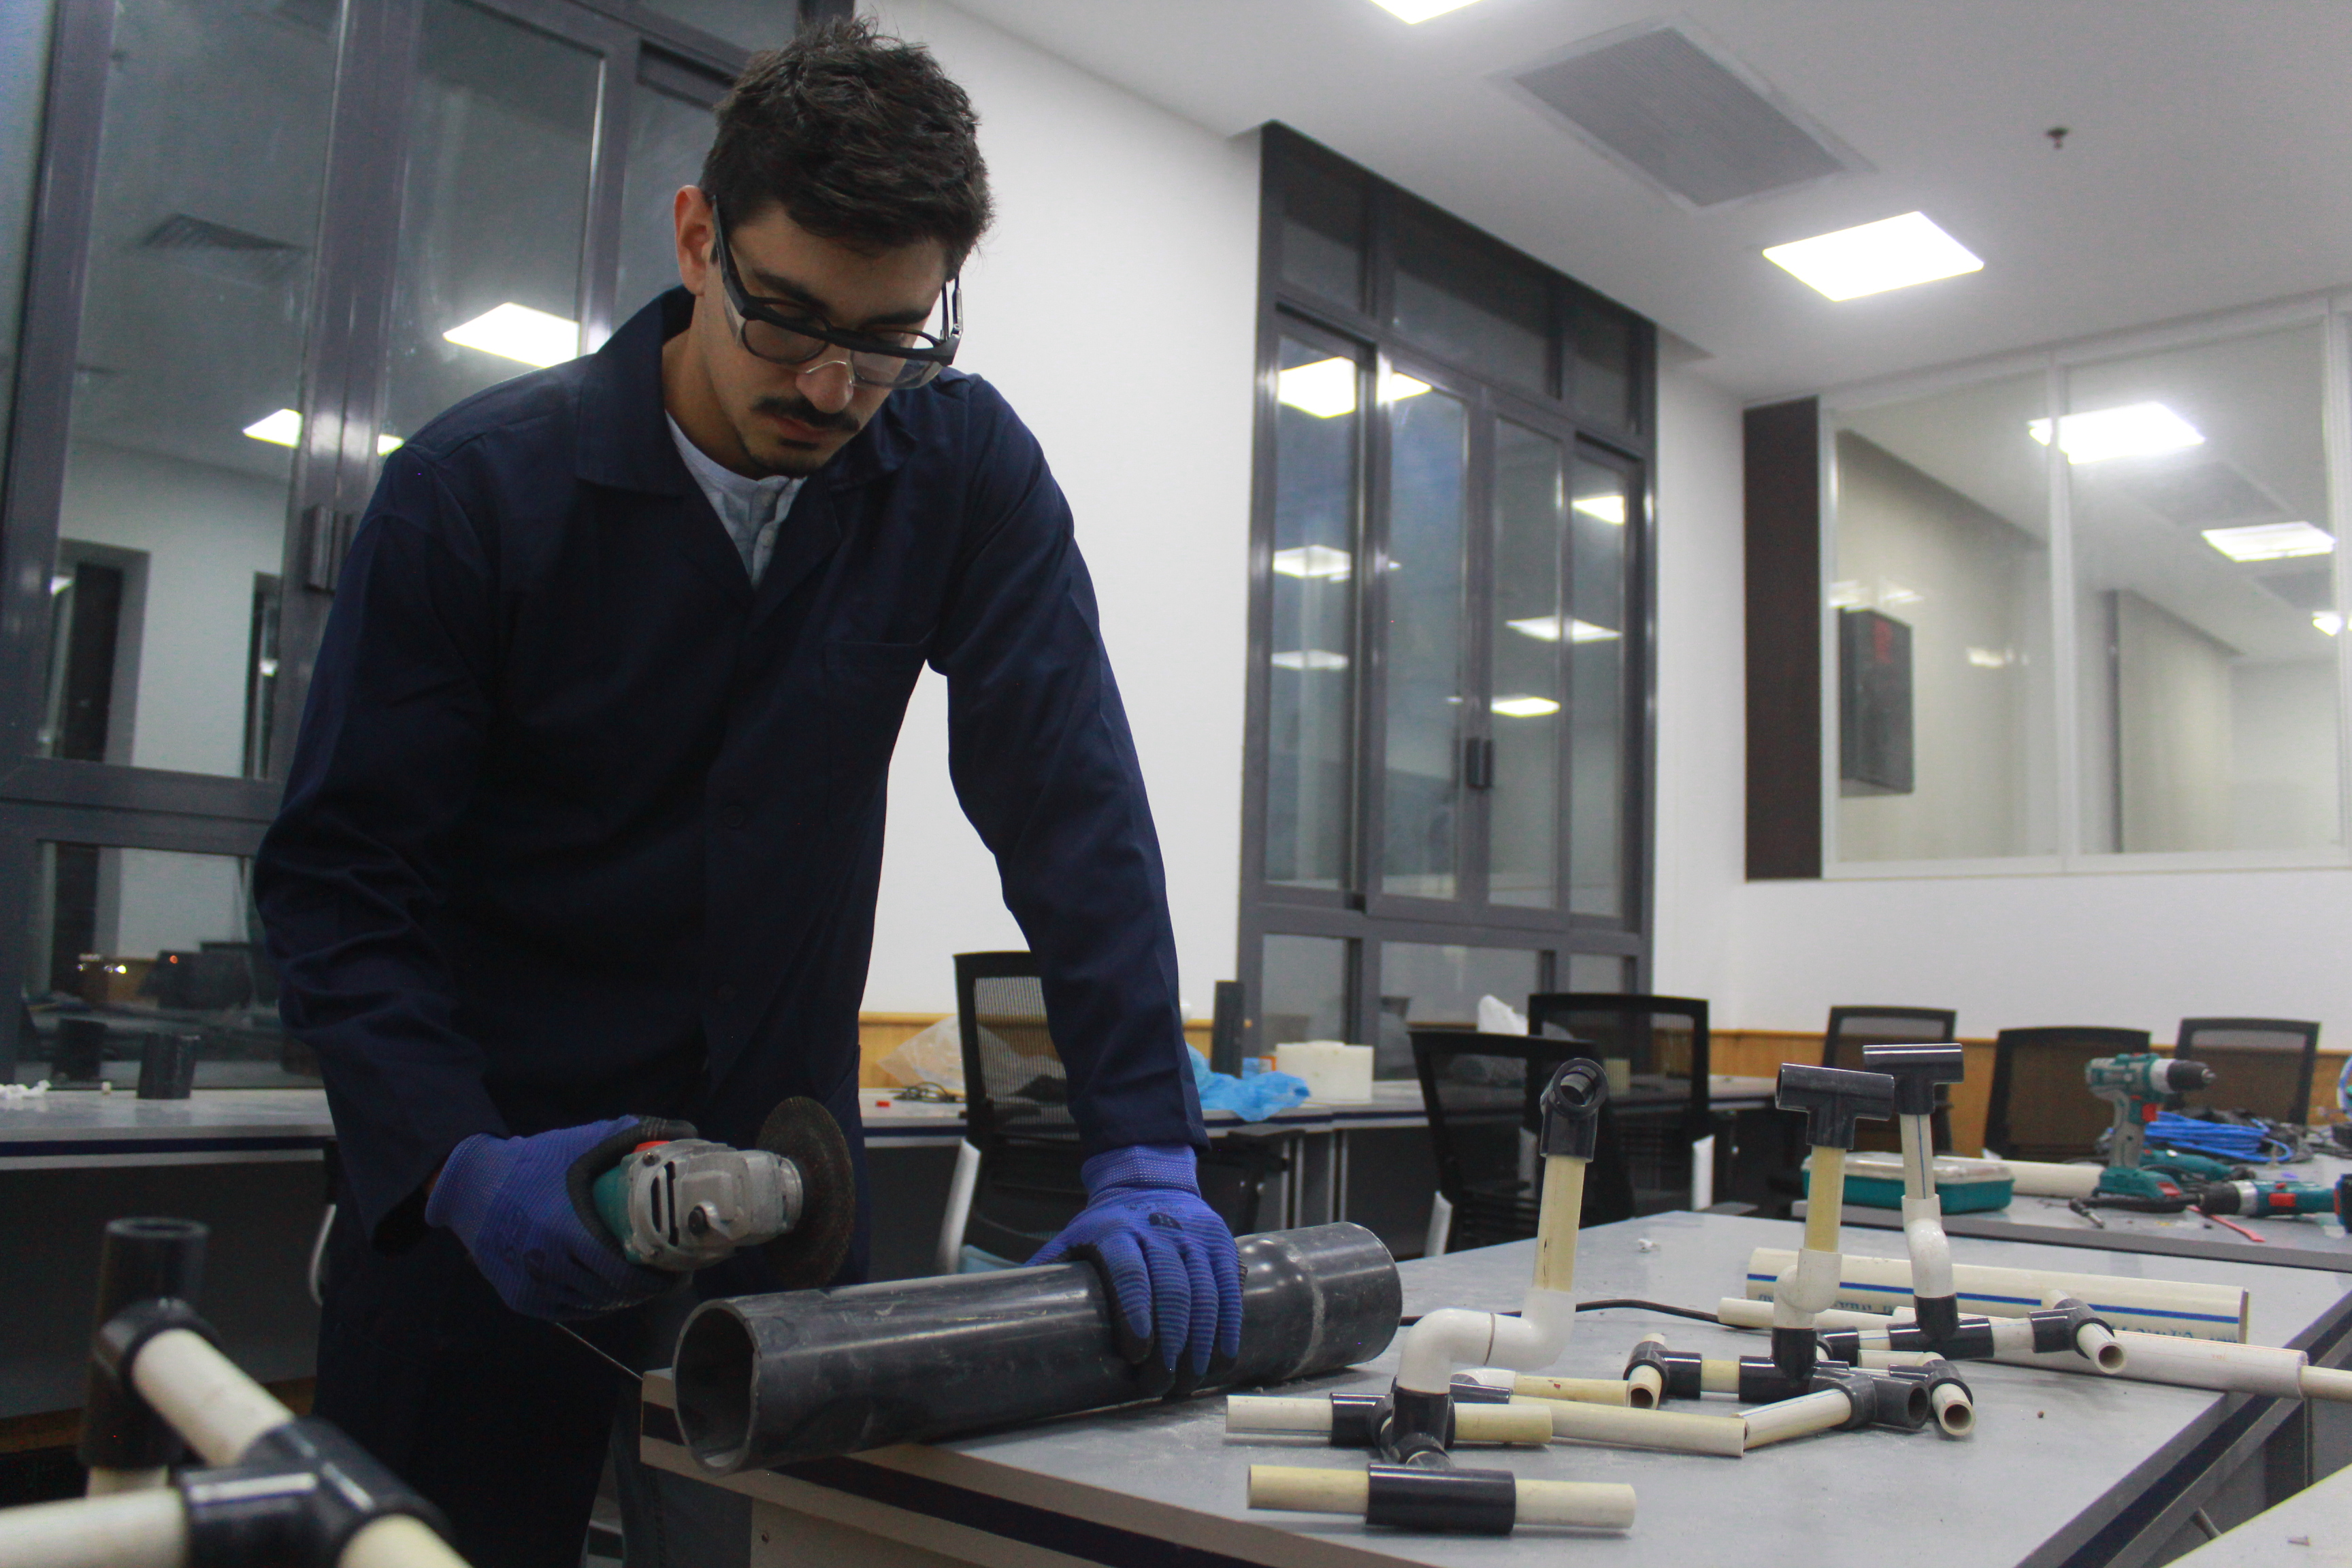
\includegraphics[width=\columnwidth]{Sections/3Safety/images/safety.jpg}
    \caption{Cutting the PVC pipes for the training track
    assembly.}
    \label{fig:safety}
\end{figure}

\subsection{Workshop Safety}

The E-JUST Robotics Club recognizes the potential dangers and hazards inherent in assembling robotics, whether mechanical or electrical. Consequently, the club has put in place strict safety procedures to ensure the security of every member. In addition, a variety of safety gear is provided in the workshop, such as soldering fume extractors, protective gloves, and face guards. All operations are supervised by a professional safety director who makes sure that the extensive safety checklist found in Appendix \ref{app:construction_checklist} is strictly followed.


\subsection{Safety Training}

In addition to receiving technical instruction, new members receive extensive safety training from experienced peers. All members acquire expertise in the procedures required to always guarantee safety through com prehensive safety training and hands-on experience obtained in a supervised environment.


\subsection{Kamikaze Safety Features}

Safety remains a top priority for the E-JUST Robotics Club, which is reflected in the design and production of Kamikaze. In compliance with MATE Organization requirements, a properly sized fuse is installed at the Anderson connectors. Strain relief is applied at both ends of the tether to prevent stress on connectors and ensure uninterrupted communication.

All bolts are securely covered, and the frame is carefully sanded to eliminate sharp edges. Kamikaze’s thrusters are equipped with protective shrouds (Figure \ref{fig:shrouds}) to enhance operator and handler safety. Additionally, its manipulators and auxiliary equipment feature extra safety measures, with Neoprene coverings ensuring a firm grip while preventing damage to nearby objects during transportation.

\begin{figure}[h]
    \centering
    \rule{0.8\columnwidth}{4cm}
    \caption{Shrouded Thrusters.}
    \label{fig:shrouds}
\end{figure}

\vspace{-0.2cm}
Each thruster operating in the aquatic environment is protected by a fuse to minimize electrical shock risks and prevent damage. For efficient heat dissipation, converters are positioned outside the canister and fully insulated, while heat-conducting components inside the canister are attached to its walls to create a heat sink effect. This design effectively manages temperatures and ensures optimal system performance.


\subsection{Safety Checklist}

All members participating in Kamikaze’s deployment must follow a strict safety procedure enforced by the E-JUST Robotics Club. Routine inspections are conducted, and Appendix \ref{app:operational_safety_checklist} outlines a comprehensive operating safety standard. While all members are responsible for adhering to the safety checklist, its strict implementation is supervised by a trained safety director.


\section{Testing and Troubleshooting}

\subsection{Full System Testing}


\subsection{Mechanical Testing}

To ensure maximum reliability, safety, and performance, Kamikaze’s mechanical system underwent a comprehensive and rigorous testing process. This approach ensured seamless operation under challenging underwater conditions, minimized the risk of failure, and upheld high safety standards.

\hspace{10pt} From the initial design phase, all components were carefully developed with a strong focus on safety, integration, and effectiveness. Before moving on to the final design and manufacturing stage, every prototype was thoroughly tested and refined to ensure flawless incorporation into Kamikaze’s final structure.

\vspace{-0.5\baselineskip}
\begin{itemize}
    \setlength{\itemsep}{0pt}
    \item \textbf{Pneumatic System Testing:} To ensure the reliability and performance of the pneumatic manipulators, a series of targeted tests were conducted. All pneumatic hoses, joints, and fittings were visually inspected to ensure proper assembly and tight sealing. The system was then pressurized, and any air leakage was detected by listening to hissing sounds particularly at fittings and connectors. Any issues were promptly resolved to ensure leak-free, efficient pneumatic actuation.
    \item \textbf{Sealing Mechanism Testing:} The electronic enclosure's sealing was tested under pressure conditions similar to those expected during operation. The enclosure was submerged and weighed underwater to check for any water ingress. If a leak was observed, compressed air was introduced into the enclosure, and the source of the leakage was identified by monitoring escaping bubbles. This allowed for targeted repairs and ensured complete waterproofing.
\end{itemize}

These mechanical and functional tests were complemented by a structured troubleshooting methodology, including:

\vspace{-0.5\baselineskip}
\begin{itemize}
    \setlength{\itemsep}{0pt}
    \item Component isolation to identify faulty subsystems.
    \item Visual inspections and real-time monitoring during tests.
    \item Failure mode analysis to understand and mitigate risks.
\end{itemize}




\section{Logistics}

\subsection{Company History}

Founded in 2021 at Egypt-Japan University of Science and Technology (E-JUST), the club began with courses and workshops to support robotics learners. Over time, members engaged in large-scale projects, forming specialized teams for competitions.

\hspace{10pt} A major milestone was the \textbf{formation of the first ROV team in 2023}, which competed in MATE ROV 2023 and won the \textbf{"No Pain, No Gain"} award. The team improved further in MATE ROV 2024, excelling in underwater tasks.

\hspace{10pt} The club unites students from various fields, following a structured training process to ensure knowledge transfer and skill development:
\vspace{-0.5\baselineskip}
\begin{enumerate}[leftmargin=0pt, itemindent=20pt]
    \setlength{\itemsep}{0pt}
    \item \textbf{General Training:} New members learn robotics fundamentals, including design, electronics, programming, and control.
    \item \textbf{Evaluation:} Members are assessed to identify strengths and roles.
    \item \textbf{Team Selection:} Based on performance, members join the ROV or other teams.
\end{enumerate}

The E-JUST ROV team has \textbf{47 members} divided into:
\vspace{-0.5\baselineskip}
\begin{itemize}[leftmargin=0pt, itemindent=20pt]
    \setlength{\itemsep}{0pt}
    \item \textbf{Technical Sector:} Focuses on ROV design and development.
    \item \textbf{Non-Technical Sector:} Manages operations and outreach.
\end{itemize}
This year, the team developed \textbf{Kamikaze}, our custom ROV, using Agile methodology and cloud-based collaboration.

\subsection{Company Structure}

Company structure is shown in Figure \ref{fig:company_structure}.

\begin{figure}[h]
    \centering
    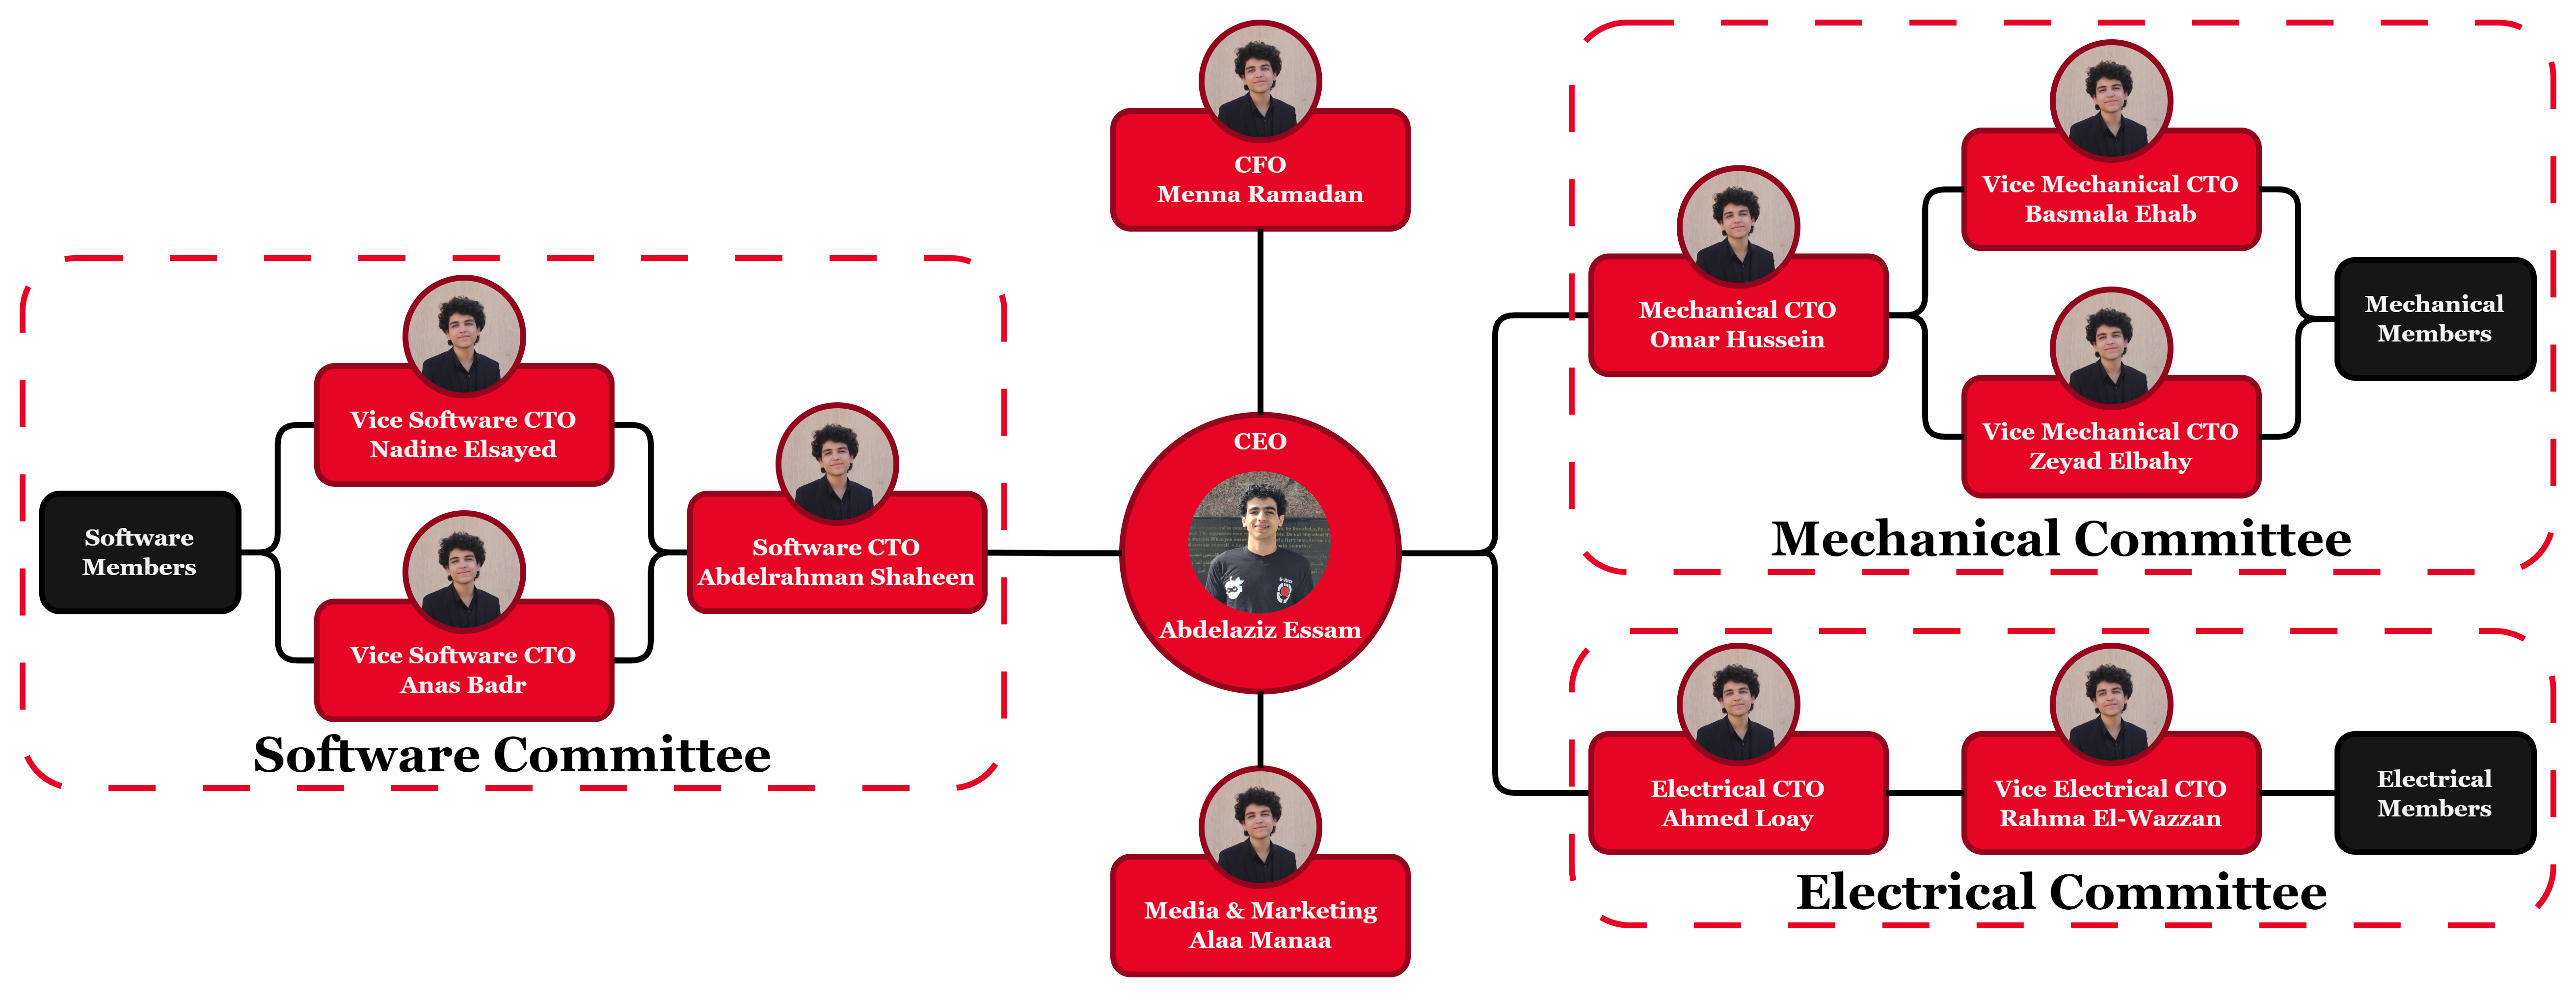
\includegraphics[width=\columnwidth]{Sections/5Logistics/images/ROV hierarchy.png}
    \caption{Company Structure.}
    \label{fig:company_structure}
\end{figure}

\textbf{Team Board}
\vspace{-0.5\baselineskip}
\begin{itemize}[leftmargin=0pt, itemindent=20pt]
    \setlength{\itemsep}{0pt}
    \item \textbf{CEO (Chief Executive Officer):} Oversees all activities and high-level decision-making.
    \item \textbf{CFO (Chief Financial Officer):} Manages budget, funding, and financial operations.
\end{itemize}

\textbf{Technical Sector}

The technical sector has three divisions, each led by a CTO (Chief Technical Officer) and Vice CTOs:
\vspace{-0.5\baselineskip}
\begin{enumerate}[leftmargin=0pt, itemindent=20pt]
    \setlength{\itemsep}{0pt}
    \item \textbf{Mechanical Committee:} Responsible for designing and manufacturing the physical structure of Kamikaze.
    \item \textbf{Electrical Committee:} Develops and integrates power distribution and control systems.
    \item \textbf{Software Committee:} Focuses on control algorithms, vision processing, and system automation.
\end{enumerate}

\textbf{Non-Technical Sector}

Beyond technical development, the Non-Technical Team plays a key role in logistics, outreach, and team operations:
\vspace{-0.5\baselineskip}
\begin{itemize}[leftmargin=0pt, itemindent=20pt]
    \setlength{\itemsep}{0pt}
    \item \textbf{Logistics:} Plans events and coordinates resources.
    \item \textbf{PR:} Manages communications and partnerships.
    \item \textbf{Media \& Marketing:} Creates content and manages social media.
    \item \textbf{Sponsorship \& Fundraising:} Secures funding and sponsors.
    \item \textbf{Event Management:} Organizes workshops and outreach.
\end{itemize}


\subsection{Project Management}

\subsubsection{Project Scheduling}

The vehicle development schedule has four phases (Further illustrated in Appendix \ref{app:project_plan}):

\vspace{-0.5\baselineskip}
\begin{enumerate}[leftmargin=0pt, itemindent=20pt]
    \setlength{\itemsep}{0pt} 
    \item \textbf{Training Phase (12 weeks, Aug 1 - Oct 16, 2024)}
    
    \vspace{-0.5\baselineskip}
    \begin{itemize}[leftmargin=0pt, itemindent=20pt]
        \setlength{\itemsep}{0pt} 
        \item Foundational and specialized training in software, mechanical, and electrical systems.
        \item ROV-specific training, task automation, and mock challenges.
    \end{itemize}
    \item \textbf{Planning Phase (2 weeks, Oct 17 - Oct 31, 2024)}
    \vspace{-0.8cm}
    \begin{itemize}[leftmargin=0pt, itemindent=20pt]
        \setlength{\itemsep}{0pt}
        \item Finalize designs, select components, and define software and electrical frameworks.
    \end{itemize}
    \item \textbf{Prototype Build \& Testing (19 weeks, Nov 1, 2024 - Mar 14, 2025)}
    \vspace{-0.5\baselineskip}
    \begin{itemize}[leftmargin=0pt, itemindent=20pt]
        \setlength{\itemsep}{0pt} 
        \item Mechanical assembly, electrical integration, and software implementation.
        \item Underwater testing, and system integration.
    \end{itemize}
    \item \textbf{Final Preparation \& Mock Competitions (Feb 21 - Mar 14, 2025)}
    
    \vspace{-0.5\baselineskip}
    \begin{itemize}[leftmargin=0pt, itemindent=20pt]
        \setlength{\itemsep}{0pt} 
        \item Simulate competition tasks and finalize adjustments. Prepare for transport and setup.
    \end{itemize}
\end{enumerate}
The schedule ensures a structured development process for a fully tested ROV.

\subsubsection{Resource Management}

\vspace{-0.5\baselineskip}
\begin{itemize}[leftmargin=0pt, itemindent=20pt]
    \setlength{\itemsep}{0pt}
    \item \textbf{Custom vs. Commercial Solutions:} We developed custom ESCs, a USB Hub, a Square Canister, and manipulators for integration, performance, and cost efficiency.
    \item \textbf{Cloud-Based Collaboration:}
    \vspace{-0.5\baselineskip}
    \begin{itemize}
        \setlength{\itemsep}{0pt}
        \item Cloud storage enabled sharing of design files and task submissions for remote collaboration.
        \item Altium shared models ensured access to the latest PCB designs.
    \end{itemize}
\end{itemize}

\subsubsection{Procedures \& Workflow}

\vspace{-0.5\baselineskip}
\begin{itemize}[leftmargin=0pt, itemindent=20pt]
    \setlength{\itemsep}{0pt}
    \item \textbf{Agile Development Approach:}
    \vspace{-0.5\baselineskip}
    \begin{itemize}[leftmargin=0pt, itemindent=20pt]
        \setlength{\itemsep}{0pt}
        \item \textbf{\textit{Agile methodology}} promoted collaboration and modularity.
        \item \textbf{\textit{Notion}} managed sprint planning, tracked tasks, and documented our work.
    \end{itemize}
    \item \textbf{Communication \& Coordination:}
    \vspace{-0.5\baselineskip}
    \begin{itemize}[leftmargin=0pt, itemindent=20pt]
        \setlength{\itemsep}{0pt}
        \item Weekly Online Meetings: Weekly virtual meetings via \textbf{\textit{Discord}} allowed real-time updates.
        \item \textbf{\textit{Miro}} for Visualization: Used for mind maps and flowcharts. 
        \item \textbf{\textit{Overleaf}} for Documentation: Enabled efficient collaboration.
        \item \textbf{\textit{GitHub}} for development: Managed (CI/CD), version control, and issue tracking.
    \end{itemize}
\end{itemize}

\subsubsection{Protocols \& Problem-Solving}
\vspace{-0.5\baselineskip}
\begin{itemize}[leftmargin=0pt, itemindent=20pt]
    \setlength{\itemsep}{0pt}
    \item \textbf{Safety \& Reliability:} Strict testing ensured safe underwater operation.
    \item \textbf{Code \& Hardware Optimization:}
    \vspace{-0.5\baselineskip}
    \begin{itemize}[leftmargin=0pt, itemindent=20pt]
        \setlength{\itemsep}{0pt}
        \item \textbf{\textit{GitHub}} enabled parallel software development and version tracking.
        \item Custom hardware optimized power efficiency.
    \end{itemize}
    \item \textbf{Issue Tracking \& Contingency Planning:}
    \vspace{-0.5\baselineskip}
    \begin{itemize}[leftmargin=0pt, itemindent=20pt]
        \setlength{\itemsep}{0pt}
        \item \textbf{\textit{Notion}} documented technical challenges and solutions.
        \item \textbf{\textit{Miro’s}} visualization tools assisted in analyzing issues.
    \end{itemize}
\end{itemize}

By integrating Agile workflows, cloud-based collaboration, real-time communication, and custom-built hardware, we ensured Kamikaze met its objectives.

\subsection{Budget and Accounting}

E-just Robotics operates within a limited self-funded budget and relies primarily on university funds. Therefore, it is crucial to use these resources judiciously to avoid unnecessary expenses. To oversee this, a Chief Financial Officer (CFO) manages all financial aspects, including budget setting and ensuring efficient utilization of the company's financial resources.

\hspace{10pt} Additionally, Egypt currently experiences a high inflation rate, which diminishes the purchasing power of the same amount of funds. 

\hspace{10pt} More detailed budget breakdowns can be found in Appendices \ref{app:budget} and \ref{app:cost_breakdown}.


\section{Conclusion}

\subsection{Future Improvements}


\subsection{Acknowledgements}

E-JUST Robotics Club would like to extend our gratitude to E-JUST 
\begin{figure}[h]
  \centering
  
\includegraphics[width=0.75\columnwidth]{Sections/6Conclusion/images/ejust_logo.png}
  \caption{E-JUST Logo}
  \label{fig:example2}
\end{figure}
for its unwavering technical and financial support since our inception. Special appreciation goes to Prof. Amr Adly, the university president, and Prof. Amr B. Eltawil, the dean of the School of Innovative Design Engineering, for their continuous support. We also acknowledge the invaluable contribution of the mechatronics department and our technical supervisors:
\begin{itemize}
    \setlength{\itemsep}{0pt}
    \item Dr. Victor Parque, Visiting Professor from Waseda University.
    \item Dr. Haitham El-Hussieny, Associate Professor.
\end{itemize}
We would also like to thank:
\begin{itemize}
    \setlength{\itemsep}{0pt}
    \item MATE for organizing such an amazing competition.
    \item AAST for coordinating the regional competition.
    \item SolidWorks and Altium for sponsoring us with student licenses.
\end{itemize}

\begin{figure}[h]
    \centering
    \begin{subfigure}[b]{0.2\textwidth}
        \centering
        
\includegraphics[width=0.55\textwidth]{Sections/6Conclusion/images/MATE_logo.png}
        \caption{MATE Logo}
    \end{subfigure}
    \begin{subfigure}{0.2\textwidth}
        \centering
        
\includegraphics[width=0.55\textwidth]{Sections/6Conclusion/images/AAST_logo.png}
        \caption{AAST Logo}
    \end{subfigure}
    \begin{subfigure}[b]{0.2\textwidth}
        \centering
        
\includegraphics[width=0.75\textwidth]{Sections/6Conclusion/images/solidworks_logo.png}
        \caption{SolidWorks Logo}
    \end{subfigure}
    \begin{subfigure}[b]{0.2\textwidth}
        \centering
        
\includegraphics[width=0.75\textwidth]{Sections/6Conclusion/images/altium_logo.png}
        \caption{Altium Logo}
    \end{subfigure}
    \caption{Logos of MATE, AAST, SolidWorks, and Altium.}
    \label{fig:logos}
\end{figure}

\subsection{References}

\nocite{*}
\printbibliography[heading=none]


\section{Appendix}
\appendix

\section{SIDs} \label{app:sids}

\subsection{Fluid SID} \label{app:fluid_sid}

\begin{figure}[h!]
    \centering
    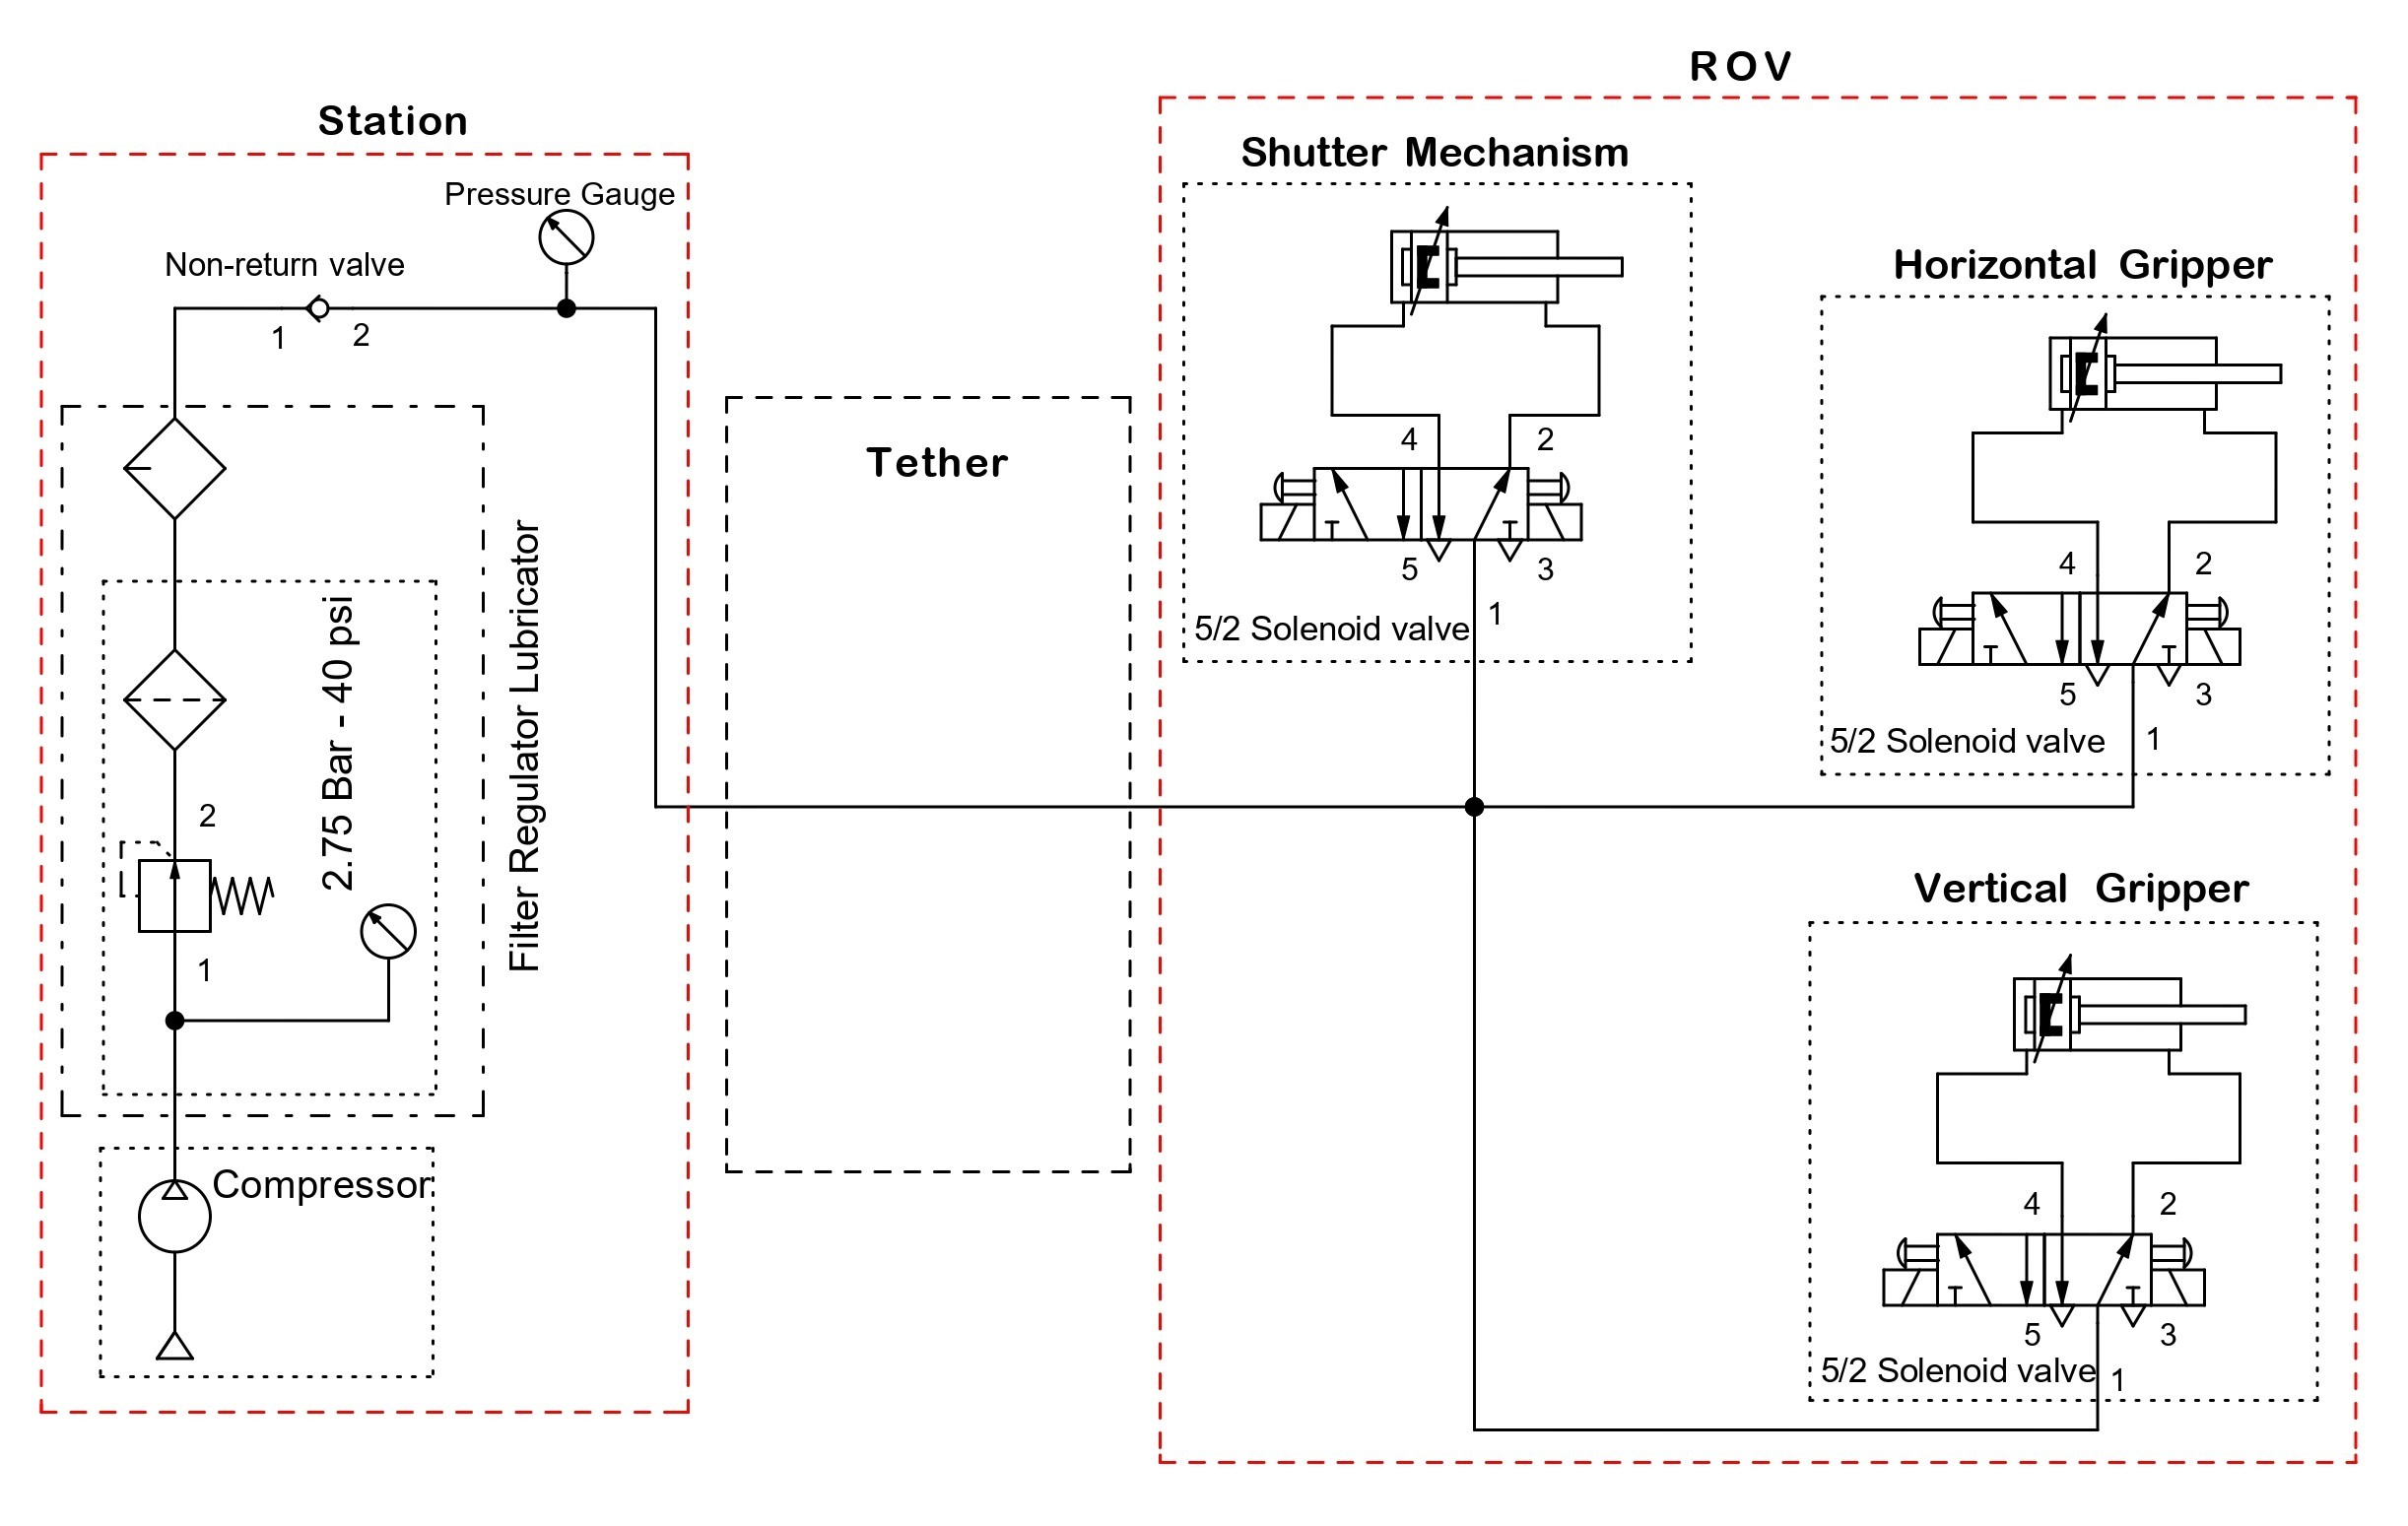
\includegraphics[width=\columnwidth]{Sections/7Appendicies/images/Pneumatic SID.jpg}
    \caption{Pneumatic SID.}
    \label{fig:pneumatic_sid}
\end{figure}

\subsection{Electrical SID}



\section{Construction Checklist} \label{app:construction_checklist}

\begin{itemize}[label=\ding{111}, leftmargin=0pt, itemindent=15pt]
    \setlength{\itemsep}{0pt}
    \item Ensure that appropriate personal protective equipment (PPE) such as gloves, goggles, and earmuffs are worn during all tasks.
    \item Sharp tools and equipment are stored properly when not in use, with blades covered or secured in racks or containers to prevent accidental cuts or injuries.
    \item Regularly check and maintain emergency kits, including fire extinguishers and first-aid supplies.
    \item Clearly label and store hazardous materials separately to ensure safe handling.
    \item Handle sharp tools with care, store them securely when not in use, and cover sharp edges with caps if available.
    \item Emergency response procedures are clearly outlined and accessible, including the location and condition of fire extinguishers, first aid kits, and emergency contact information.
    \item Maintain well-ventilated work areas and use additional fume extractors to prevent inhalation of harmful fumes while working with materials such as epoxy and soldering.
    \item Electrical components and wiring are handled with care, following proper insulation and grounding procedures to prevent electrical shocks or short circuits.
\end{itemize}

\section{Operational Safety Checklist} \label{app:operational_safety_checklist}

\subsection{Pre-Deployment}
\begin{itemize}[label=\ding{111}, leftmargin=0pt, itemindent=15pt]
    \setlength{\itemsep}{0pt}
    \item On deck in proper safety attire.
    \item Ensure power is OFF.
    \item Clear poolside of obstructions.
    \item Confirm untangled tether connected securely with strain relief.
    \item Check tether connection to Control Unit.
    \item Verify no exposed wires or loose connections.
    \item Confirm electronics housing sealing.
    \item Ensure control computer is operational.
\end{itemize}
\subsection{Power Up}
\begin{itemize}[label=\ding{111}, leftmargin=0pt, itemindent=15pt]
    \setlength{\itemsep}{0pt} 
    \item Confirm ROV receives 48V.
    \item Perform dry tests on thrusters, manipulators, and payloads.
    \item Check all video feeds.
\end{itemize}
\subsection{Launch and Water Entry}
\begin{itemize}[label=\ding{111}, leftmargin=0pt, itemindent=15pt]
    \setlength{\itemsep}{0pt}
    \item Two members handle ROV.
    \item Tether handler holds tether.
    \item Visually inspect for leaks and air bubbles.
    \item Test thrusters, manipulators, and payloads.
\end{itemize}
\subsection{Communication Loss}
\begin{itemize}[label=\ding{111}, leftmargin=0pt, itemindent=15pt]
    \setlength{\itemsep}{0pt}
    \item Reboot ROV.
    \item Resend test package.
  
If no communication:
  
    \item Power down ROV.
    \item Retrieve ROV via tether.
    \item Check for damage or leaks.
    \item Dry Test
\end{itemize}
\subsection{Retrieval}
\begin{itemize}[label=\ding{111}, leftmargin=0pt, itemindent=15pt]
    \setlength{\itemsep}{0pt}
    \item Surface ROV and turn off thrusters.
    \item Assigned crew grab ROV by handles.
    \item Secure ROV on deck.
    \item Power down ROV and Control Unit.
\end{itemize}




\section{Budget} \label{app:budget}

\subsection{Travel Estimate}

\begin{longtblr}[
  caption = {Traveling expense breakdown.},
  label = {tab:travel_expense},
  entry = {Table \thetable},
  ]{
  width = \columnwidth,
  colspec = {| Q[c, m, wd=1.4cm] | X[l, m, wd=4.2cm] | Q[c, m, wd=1.5cm] |},
  hline{1,Z} = {solid},
  hline{2, 3, 4, 5, 6, 7, 8} = {solid},
  rows = {font=\tiny,rowsep=0pt},
  row{1} = {font=\bfseries\tiny},
  row{4, 8} = {font=\bfseries\tiny},
  column{1} = {font=\bfseries\tiny},
  }
{} & {Category} & {Expenses (USD)} \\
\SetCell[r=2]{m} Expenses per Team & Team transportations in Alpena, Michigan & 400 \\
{} & ROV Shipping & 650 \\
\SetCell[c=2]{c} Total & & 1050 \\
\SetCell[r=3]{m} Expenses per Member & Residency in Alpena, Michigan per member & 350 \\
{} & Tickets expenses per member & 1600 \\
{} & Visa Fees per member & 185 \\
\SetCell[c=2]{c} Total per member & & 2205 \\
\end{longtblr}

The number of individuals traveling to the USA will be determined based on available sponsorship opportunities, which may cover some or all of the costs. We expect to have a clear understanding of these details by June 1, 2025.

\subsection{Fundraising}
\vspace{-0.6cm}
\begin{longtblr}[
  caption = {Income breakdown.},
  label = {tab:income},
  entry = {Table \thetable}
]{
  width = \columnwidth,
  colspec = {| Q[c, m] | X[l, m] | Q[c, m, wd=1.4cm] |},
  hline{1, 2, 3, 4, 5, Z} = {solid},
  rows = {font=\tiny,rowsep=0pt},
  row{1} = {font=\bfseries\tiny},
  row{5} = {font=\bfseries\tiny}
}
{Category} & {Source} & {Cost (USD)} \\
{Sponsorship} & {E-just University fund} & {2000} \\
{Sponsorship} & {ISF fund} & {1000} \\
{Self-fund} & {By Team members} & {156} \\
\SetCell[c=2]{c} Total Income & & {3156} \\
\end{longtblr}

\vspace{-0.4cm}
\subsection{Budget Allocation}
\vspace{-0.6cm}
\begin{longtblr}[
  caption = {Budget Allocation.},
  label = {tab:budget_allocation},
  entry = {Table \thetable}
]{
  width = \columnwidth,
  colspec = {| Q[c, m, wd=1.6cm] | X[l, m, wd=4.2cm] | Q[c, m, wd=1.3cm] |},
  hline{1-Z} = {solid},
  rows = {font=\tiny,rowsep=0pt},
  row{1, 8} = {font=\bfseries\tiny},
  column{1} = {font=\bfseries\tiny}
}
{Category} & {Description} & {Cost (USD)} \\
{ROV Materials \& Machining} & {ROV tether, Cameras encapsulation, Canister} & {1080} \\
{ROV Electronics} & {power converters, cameras, etc} & {1050} \\
{Float} & {Its Structure, Electronics, and Sensors} & {400} \\
{Lab Safety} & {Safety glasses, labels, ventilation, gloves, etc.} & {70} \\
{Team Operations} & {Team branding (shirts, Logo stickers, etc)} & {275} \\
{Competition Fees} & {Registration fees for MATE ROV Competition} & {650} \\
\SetCell[c=2]{c} Total Expenses & & {3,525} \\
\end{longtblr}

\section{Cost Breakdown} \label{app:cost_breakdown}

\subsection{Reused Items}

\begin{table}[h!]
    \centering
    \renewcommand{\arraystretch}{1.2}
    \begin{adjustbox}{width=\columnwidth}
    \begin{tabular}{|>{\centering\arraybackslash}p{2.7cm}|l|>{\centering\arraybackslash}p{3cm}|>{\centering\arraybackslash}p{3cm}|}
    \hline
    \textbf{Category} & \textbf{Component} & \textbf{Quantity/Weight} & \textbf{Total Price (USD)} \\
    \hline
    \multirow{8}{*}{\textbf{Electronics}} 
     & T200 Thrusters & 6 & 2964 \\
     & ESC (Electronic Speed Controller) & 6 & 419 \\
     & Logitech C270 Widescreen HD Webcam & 3 & 109 \\
     & Water Depth/Pressure Sensor MS5540 & 1 & 17 \\
     & TP-Link TL-WR840N 300 Mbps Wireless N Router & 1 & 17 \\
     & 10 DOF IMU (MPU9250+BMP280) & 1 & 16 \\
     & ROV Controller & 1 & 20 \\
     & 12V to 5V DC-DC Converter & 3 & 148 \\
    \hline
    \multirow{2}{*}{\textbf{Tools/Supplies}}
     & Digital Multimeter & 2 & 33 \\
     & Soldering Iron 220V 100W & 2 & 17 \\
    \hline
    \multirow{5}{*}{\textbf{Pneumatics}}
     & Pressure regulator & 1 & 65 \\
     & Air Solenoid Valve 12VDC Bi-Directional & 1 & 11 \\
     & Pneumatic Cylinder MI25-25-S & 2 & 20 \\
     & Non-return Valve & 1 & 10 \\
     & Air Solenoid Valve 12VDC (5/2) & 2 & 12 \\
    \hline
    \textbf{Safety Equipment/PPE}
     & Safety Glasses, Vests, etc & -- & 10 \\
    \hline
    \multicolumn{3}{|c|}{\textbf{Total}} & 4150 \\
    \hline
    \end{tabular}
    \end{adjustbox}
    \caption{Reused components and their costs.}
    \label{tab:components}
\end{table}

The exchange rate between the U.S. dollar (USD) and Egyptian pound (EGP) is 50.57 EGP per dollar in Sun, 28 March 2025.

\newpage
\subsection{Purchased Items}

\begin{table}[hb]
    \centering
    \renewcommand{\arraystretch}{1.2}
    \begin{adjustbox}{width=\columnwidth}
    \begin{tabular}{|>{\centering\arraybackslash}p{2cm}|>{\raggedright\arraybackslash}p{9cm}|>{\centering\arraybackslash}p{2.7cm}|}
    \hline
    \textbf{Category} & \textbf{Component} & \textbf{Total Price USD} \\
    \hline
    \multirow{11}{*}{\textbf{\makecell{Mechanical\\ Material}}}
     & Artelon Sheet (10mm*1m*1m) & 76.95 \\
     & Toggle Clamp Latch & 102.94 \\
     & Transparent Acrylic Sheet (6mm*2m*1.3m) & 120.44 \\
     & 2020 extrusion & 54.56 \\
     & 2040 extrusion & 16.73 \\
     & Aluminium T-bracket & 15.44 \\
     & Aluminium L-slot bracket & 10.29 \\
     & 90 degree Aluminium plate & 16.73 \\
     & T-slot Nut & 15.44 \\
     & Allen bolt & 11.58 \\
     & Aluminium sheet & 54.56 \\
    \hline
    \multirow{16}{*}{\textbf{Electronics}}
     & ESC (Electronic Speed Controller) & 95.74 \\
     & ZED 2 Stereo Camera & 839.75 \\
     & CCTV Camera & 77.46 \\
     & Raspberry Pi 5 - 8GB RAM With Active Cooler & 193.01 \\
     & Cat 6e 50 meter & 15.93 \\
     & STM32F401RCT6 & 8.36 \\
     & Stranded Aluminum Wire - 16 mm² & 59.29 \\
     & WS2812 RGB Diffused Addressable LED 5mm 5V & 6.18 \\
     & UGREEN Braided USB to USB C & 46.32 \\
     & General purpose Mosfets & 7.72 \\
     & High Torque Servo Motor (15 kg.cm - Metal Gear) & 39.12 \\
     & STM32F411 Black Pill & 23.68 \\
     & 15mm Expandable Braided Cable Sleeve & 19.30 \\
     & Barrier Terminal Block & 12.87 \\
     & PCB Manufacturing & 102.94 \\
     & Resistors & 6.43 \\
    \hline
    \multirow{5}{*}{\textbf{Pneumatics}}
     & Pneumatic Straight fitting 6 mm & 2.51 \\
     & Air Solenoid Valve 12VDC Bi-Directional & 13.38 \\
     & Pneumatic Cylinder M125-25-S & 11.71 \\
     & Non-return Valve & 11.71 \\
     & Air Solenoid Valve 12VDC (5/2) & 7.03 \\
    \hline
    \multirow{4}{*}{\textbf{Sealing}}
     & Pneumatic Clear Hose 8*6mm & 11.37 \\
     & Sealing Blue Foam (5cm thickness) & 6.69 \\
     & Glands & 1.67 \\
     & Rubber Gaskets (1m*1m) & 11.71 \\
    \hline
    \multirow{9}{*}{\textbf{Float}}
     & Acrylic Cylinder (20 cm) & 257.35 \\
     & Stainless Lead Screw with Nut (8x1000mm) Pitch 2mm & 7.46 \\
     & Pneumatic Hose & 10.29 \\
     & Allen bolt & 3.86 \\
     & Lead Screw Nut & 0.26 \\
     & Artelon Sheet (5mm*50cm*50cm) & 15.44 \\
     & PCB Manufacturing & 77.20 \\
     & STM32F411 Black Pill & 11.84 \\
     & NI-MH Rechargeable Battery AA 1800mAh 1.2V (2PCS) & 20.07 \\
    \hline
    \multicolumn{2}{|c|}{\textbf{Total}} & 2,531.31 \\
    \hline
    \end{tabular}
    \end{adjustbox}
    \caption{Purchased Materials.}
    \label{tab:bom}
\end{table}

\end{document}